%-------------------------------------------------------------------------
% c-td-info-S1.tex
%-------------------------------------------------------------------------

%-------------------------------------------------------------------------
\documentclass[11pt,a4paper,colorlinks,breaklinks]{book}
%-------------------------------------------------------------------------

%-------------------------------------------------------------------------
\usepackage{calc}
\usepackage[text={16cm,23cm},centering=true,showframe=false]{geometry}
\usepackage{fancybox,fancyvrb,fancyhdr,lastpage,lineno,import}
\usepackage{longtable,multirow}
\usepackage{xcolor,graphics,xmpmulti,pgf,pgfpages,tikz,wrapfig}
\usepackage{colortbl,color}
\usepackage{amsmath,amssymb,amsfonts}
\usepackage{hyperref,multimedia,rotating,framed,pstricks}
\usepackage{listings,index}
%
%---- pdflatex
%\usepackage[T1]{fontenc}
%\usepackage[utf8]{inputenc}
%---- xelatex
\usepackage{fontspec}
%
%\usepackage[french]{minitoc}
\usepackage[french]{babel}
\usepackage[french]{nomencl}
\usepackage[framed,hyperref,standard]{ntheorem}
\usepackage{eurosym,pifont}
%-------------------------------------------------------------------------

%-------------------------------------------------------------------------
\definecolor{blanc}{RGB}{255,255,255}
\definecolor{orange}{RGB}{234,138,0}
\definecolor{bleu}{RGB}{144,209,223}
\definecolor{rose}{RGB}{233,96,124}
\definecolor{beige}{RGB}{247,244,241}
\definecolor{violet}{RGB}{159,159,202}
\definecolor{vert}{RGB}{162,169,63}
\definecolor{marron}{RGB}{193,181,162}
\definecolor{noir}{RGB}{62,61,64}
%-------------------------------------------------------------------------

%-------------------------------------------------------------------------
\usetikzlibrary{mindmap,backgrounds,shapes,decorations.text}
%-------------------------------------------------------------------------

%-------------------------------------------------------------------------
\pgfdeclareimage[width=3cm,interpolate=true]{logo-enib}{logo-enib}
\pgfdeclareimage[width=3cm,interpolate=true]{logo-mesr}{logo-mesr}
\pgfdeclareimage[width=3cm,interpolate=true]{logo-cti}{logo-cti}
%-------------------------------------------------------------------------

%-------------------------------------------------------------------------
\input{sigle}
%-------------------------------------------------------------------------

%-------------------------------------------------------------------------
\makeatletter
\newtheoremstyle{mybreak}%
  {\item[\rlap{\vbox{\hbox{\hskip\labelsep \theorem@headerfont
          ##1\ ##2\theorem@separator}\hbox{\strut}}}]}%
  {\item[\rlap{\vbox{\hbox{\hskip\labelsep \theorem@headerfont
          ##1\ ##2\theorem@separator {\sc ##3}}\hbox{\strut}}}]}
\makeatother
\theoremseparator{\ :\ }

\newtheorem{rem}{Remarque}[chapter]
\theoremstyle{mybreak}
\newtheorem{defin}{\color{red}Définition}[chapter]
\newtheorem{td}{\color{blue}TD}[chapter]
\newtheorem{ex}{Exemple}[chapter]
\theorembodyfont{\footnotesize}
\newframedtheorem{fig}{Fig.}[chapter]
%-------------------------------------------------------------------------

%-------------------------------------------------------------------------
\hypersetup
{
colorlinks=true,
pdftitle={Initiation à l'algorithmique},
pdfauthor={Jacques TISSEAU}
}
%-------------------------------------------------------------------------

%-------------------------------------------------------------------------
\lstset
{
language=Python,
basicstyle=\footnotesize\ttfamily,
identifierstyle=\ttfamily,
keywordstyle=\color{blue}\ttfamily,
commentstyle=\color{gray}\ttfamily,
stringstyle=\color{green}\ttfamily,
showstringspaces=false,
extendedchars=true,
numbers=left, 
numberstyle=\tiny,
frame=lines,
linewidth=0.95\textwidth,
xleftmargin=5mm
} 
%-------------------------------------------------------------------------

%-------------------------------------------------------------------------
\fvset
{
fontsize=\footnotesize,
numbers=left,
numbersep=5pt,
frame=lines
}  
%-------------------------------------------------------------------------

%-------------------------------------------------------------------------
\setlength{\oddsidemargin}{0cm}
\setlength{\evensidemargin}{0cm}
\setlength{\topmargin}{-0.75cm}
%-------------------------------------------------------------------------

%-------------------------------------------------------------------------
\makeindex
\newindex{algo}{alx}{ald}{Algorithmes}
\newindex{def}{defx}{defd}{Définitions}
\newindex{td}{tdx}{tdd}{Exercices}
%-------------------------------------------------------------------------

%-------------------------------------------------------------------------
\graphicspath{{../../fig/}}
%-------------------------------------------------------------------------

\newenvironment{py}[1]{\begin{minipage}[t]{#1}\footnotesize}{\end{minipage}}

%-------------------------------------------------------------------------
\begin{document}
%-------------------------------------------------------------------------

%-------------------------------------------------------------------------
\begin{titlepage}
%-------------------------------------------------------------------------
\thispagestyle{fancy}
\lhead{\hspace*{-2em}\begin{minipage}{5cm}
\includegraphics[width=5cm]{logo-enib}\end{minipage}}
\rhead{Cours d'Informatique S1}
\setlength{\headheight}{79pt}
\setlength{\footskip}{20pt}
\renewcommand{\headrulewidth}{0pt}
\renewcommand{\footrulewidth}{0pt}

\begin{center}
{\huge\bf Initiation à l'algorithmique}\\[5mm]
{\huge\sc Solutions des travaux dirigés}\\[1cm]
\href{http://www.enib.fr/~tisseau}{\Large\sc Jacques TISSEAU}\\[3mm]
\href{http://www.enib.fr}{Ecole nationale d'ingénieurs de Brest}\\
\href{http://www.cerv.fr}{Centre européen de réalité virtuelle}\\
\href{mailto:tisseau@enib.fr}{\tt tisseau@enib.fr}
\end{center}

{\footnotesize\vspace*{1.5mm}
\noindent Avec la participation de 
{\sc Romain Bénard}, 
{\sc Stéphane Bonneaud}, {\sc Cédric Buche},
{\sc Gireg Desmeulles}, {\sc Céline Jost}, 
{\sc Sébastien Kubicki}, {\sc Eric Maisel}, 
{\sc Aléxis Nédélec}, {\sc Marc Parenthoën} et 
{\sc Cyril Septseault}.
}
\vspace*{1cm}

\noindent Ce document regroupe les solutions, testées avec \python\ 3.2.2,
des exercices du cours d'Infor\-ma\-tique 
du $1^{er}$ semestre (S1) de l'Ecole Nationale d'Ingénieurs 
de Brest (\href{http://www.enib.fr}{\enib : {\tt www.enib.fr}}). Il
accompagne les notes de cours « Initiation à l'algorithmique ».
$$\fbox{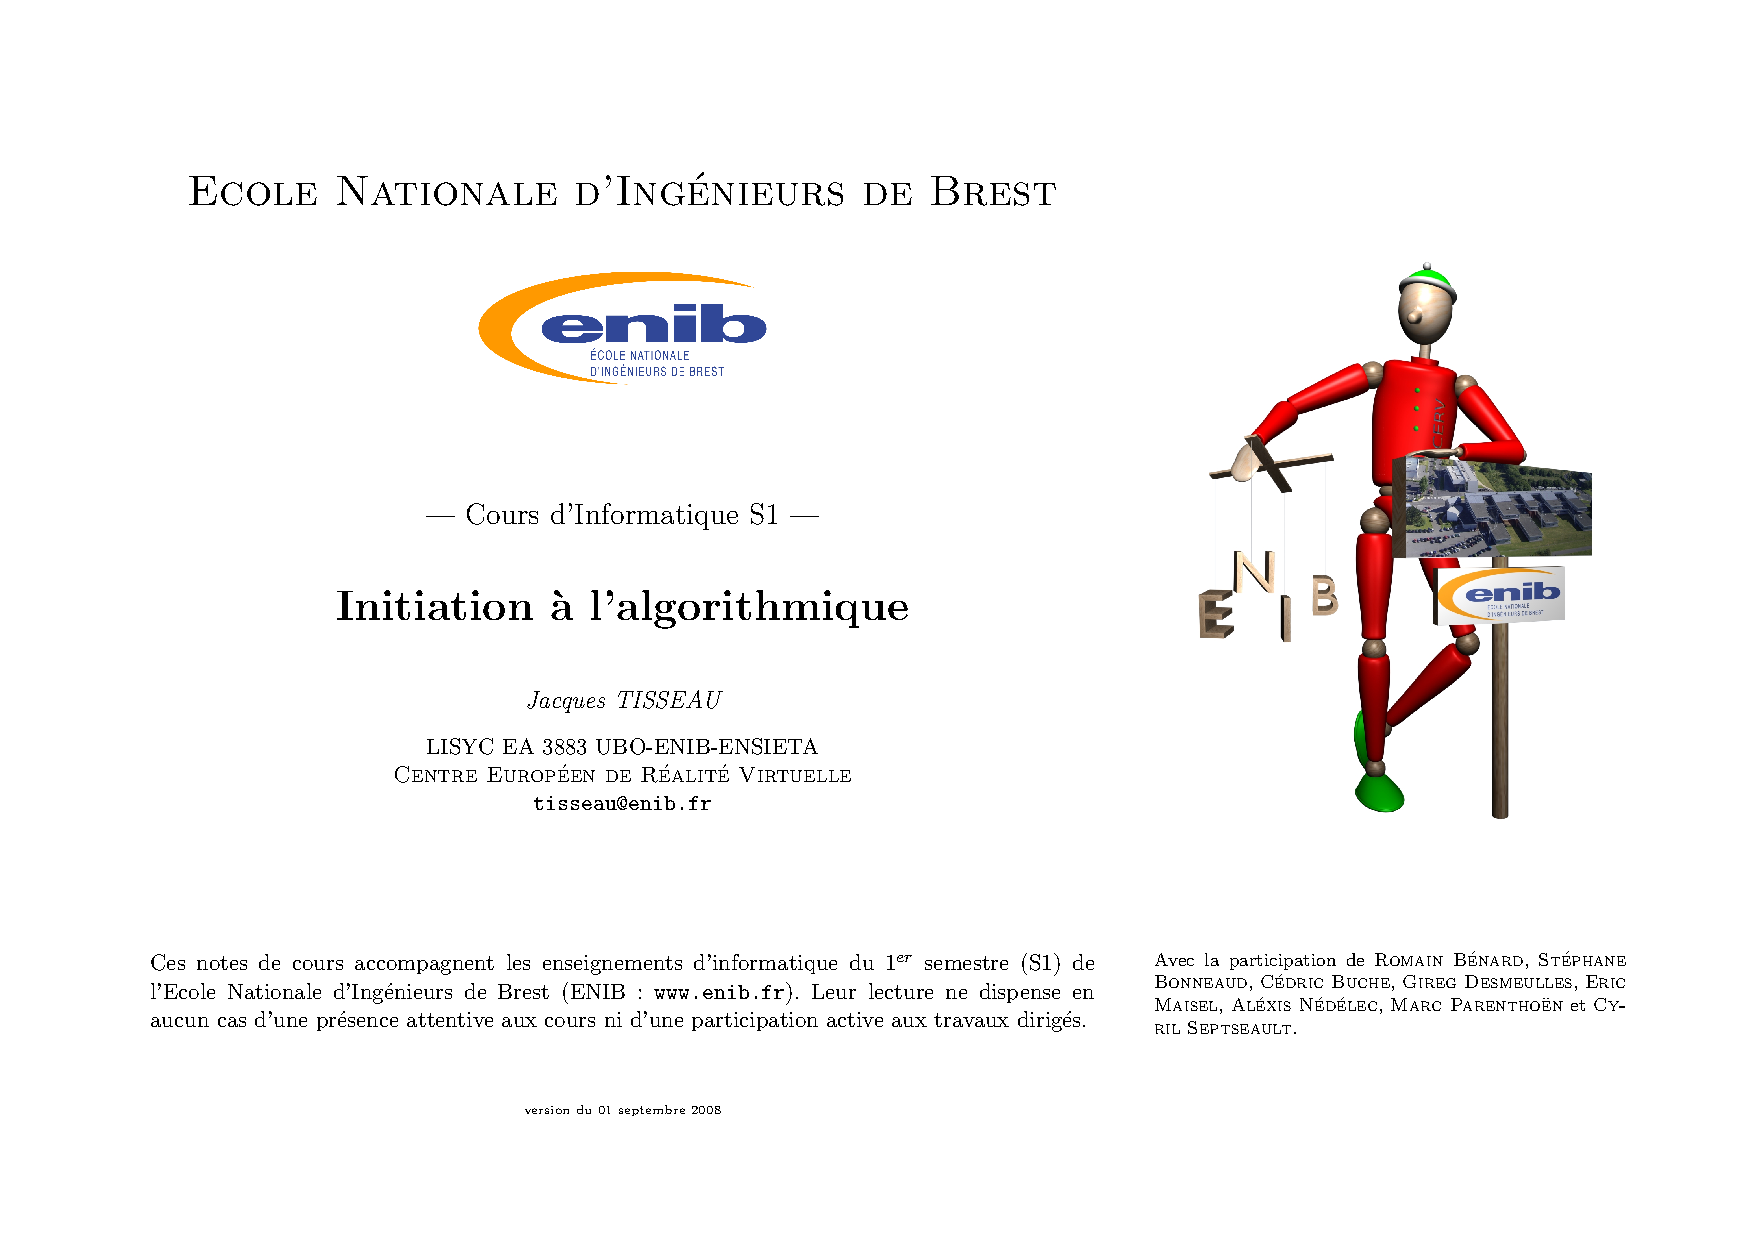
\includegraphics[width=0.9\textwidth,page=1]{../../cours/info-S1.pdf}}$$
\centerline{\footnotesize
{\bf Tisseau J.},{\em Initiation à l'algorithmique}, ENIB, cours d'Informatique S1, Brest, 2009.
}
\null\vfill

\centerline{\tiny version du \today}
\end{titlepage}
%-------------------------------------------------------------------------


%-------------------------------------------------------------------------
\renewcommand{\contentsname}{Sommaire}
\tableofcontents
%-------------------------------------------------------------------------

%-------------------------------------------------------------------------
\chapter{Introduction générale}\label{ch:introduction}
%-------------------------------------------------------------------------
	% c-td-info-S1-introduction.tex

Les exercices de ce chapitre d'introduction ne nécessitent pas
de solutions écrites en \python.
Cependant, lorsque la solution \python\ ne fait appel
qu'à des instructions aussi simples que celles d'une calculette 
(\tdir\ \ref{td:octets}, \ref{td:python})
ou celles de la tortue \logo\ (\tdir\ \ref{td:plage1}, \ref{td:plage2}, \ref{td:plage5},
\ref{td:attention1}, \ref{td:plage3}, \ref{td:tortue}), celle-ci est proposée afin de se
familiariser avec \python.
\vspace*{2mm}

%-------------------------------------------------------------------------

\begin{td}[Dessins sur la plage : exécution (1)]\label{td:plage1}
	\em\mbox{}\\[-1.2cm]
	%\em\mbox{}\hfill\begin{minipage}{0.95\textwidth}
	\VerbatimInput{td1/td1.01.py}
	%\end{minipage}
	\vspace*{2mm}
	
\end{td}

\begin{td}[Dessins sur la plage : conception (1)]\label{td:plage2}
	\em\mbox{}\\[-1.2cm]
	%\em\mbox{}\hfill\begin{minipage}{0.95\textwidth}
	\VerbatimInput{td1/td1.02.py}
	%\end{minipage}
	\vspace*{2mm}
	
\end{td}


\begin{td}[Propriétés d'un algorithme]\label{td:propPlage}
	\em\mbox{}\\[-1.2cm]
	%\em\mbox{}\hfill\begin{minipage}{0.95\textwidth}
	\VerbatimInput{td1/td1.03.py}
	%\end{minipage}
	\vspace*{2mm}
	
\end{td}


\begin{td}[Unités d'information]\label{td:octets}\index[td]{unités d'information}
	\em\mbox{}\\[-1.2cm]
	%\em\mbox{}\hfill\begin{minipage}{0.95\textwidth}
	\VerbatimInput{td1/td1.04.py}
	%\end{minipage}
	\vspace*{2mm}
	
\end{td}

\begin{td}[Première utilisation de {\sc Python}]\label{td:python}\index[td]{{{\sc Python}}}
	\em\mbox{}\\[-1.2cm]
	%\em\mbox{}\hfill\begin{minipage}{0.95\textwidth}
	\VerbatimInput{td1/td1.05.py}
	%\end{minipage}
	\vspace*{2mm}
	
\end{td}

\begin{td}[Erreur de syntaxe en {\sc Python}]\label{td:erreur}\index[td]{{{\sc Python}}}
	\em\mbox{}\\[-1.2cm]
	%\em\mbox{}\hfill\begin{minipage}{0.95\textwidth}
	\VerbatimInput{td1/td1.06.py}
	%\end{minipage}
	\vspace*{2mm}
	
\end{td}
	
\begin{td}[Dessins sur la plage : persévérance]\label{td:plage5}\index[td]{dessins sur la plage}
	\em\mbox{}\\[-1.2cm]
	%\em\mbox{}\hfill\begin{minipage}{0.95\textwidth}
	\VerbatimInput{td1/td1.07.py}
	%\end{minipage}
	\vspace*{2mm}
	
\end{td}
	
\begin{td}[Autonomie]\label{td:autonomie}\index[td]{autonomie}
	\em\mbox{}\\[-1.2cm]
	%\em\mbox{}\hfill\begin{minipage}{0.95\textwidth}
	\VerbatimInput{td1/td1.08.py}
	%\end{minipage}
	\vspace*{2mm}
	
\end{td}

\begin{td}[Site {\sc Web} d'Informatique S1]\label{td:site}\index[td]{site {{\sc Web}}}
	\em\mbox{}\\[-1.2cm]
	%\em\mbox{}\hfill\begin{minipage}{0.95\textwidth}
	\VerbatimInput{td1/td1.09.py}
	%\end{minipage}
	\vspace*{2mm}
	
\end{td}


\begin{td}[Exemple de contrôle d'attention (1)]\label{td:attention1}\index[td]{contrôle d'attention}
	\em\mbox{}\\[-1.2cm]
	%\em\mbox{}\hfill\begin{minipage}{0.95\textwidth}
	\VerbatimInput{td1/td1.10.py}
	%\end{minipage}
	\vspace*{2mm}
	
\end{td}


\begin{td}[Exemple de contrôle de TD]\label{td:TD}\index[td]{contrôle de TD}
	\em\mbox{}\\[-1.2cm]
	%\em\mbox{}\hfill\begin{minipage}{0.95\textwidth}
	\VerbatimInput{td1/td1.11.py}
	%\end{minipage}
	\vspace*{2mm}
	
\end{td}
	
\begin{td}[Exemple de contrôle d'autoformation (1)]\label{td:bool}\index[td]{contrôle d'autoformation}
	\em\mbox{}\\[-1.2cm]
	%\em\mbox{}\hfill\begin{minipage}{0.95\textwidth}
	\VerbatimInput{td1/td1.12.py}
	%\end{minipage}
	\vspace*{2mm}
	
\end{td}
	
\begin{td}[Exemple de contrôle des compétences]\label{td:competences}\index[td]{contrôle des compétences}
	\em\mbox{}\\[-1.2cm]
	%\em\mbox{}\hfill\begin{minipage}{0.95\textwidth}
	\VerbatimInput{td1/td1.13.py}
	%\end{minipage}
	\vspace*{2mm}
	
\end{td}

\begin{td}[Nombre de contrôles]\label{td:controles}\index[td]{nombre de contrôles}
	\em\mbox{}\\[-1.2cm]
	%\em\mbox{}\hfill\begin{minipage}{0.95\textwidth}
	\VerbatimInput{td1/td1.14.py}
	%\end{minipage}
	\vspace*{2mm}
	
\end{td}

\begin{td}[Exemple de contrôle d'autoformation (2)]\label{td:negation}\index[td]{contrôle d'autoformation}
	\em\mbox{}\\[-1.2cm]
	%\em\mbox{}\hfill\begin{minipage}{0.95\textwidth}
	\VerbatimInput{td1/td1.15.py}
	%\end{minipage}
	\vspace*{2mm}
	
\end{td}

\begin{td}[Exemple de contrôle d'attention (2)]\label{td:attention2}\index[td]{contrôle d'attention}
	\em\mbox{}\\[-1.2cm]
	%\em\mbox{}\hfill\begin{minipage}{0.95\textwidth}
	\VerbatimInput{td1/td1.16.py}
	%\end{minipage}
	\vspace*{2mm}
	
\end{td}

\begin{td}[Nombres d'exercices de TD]\label{td:exercices}\index[td]{nombres d'exercices de TD}
	\em\mbox{}\\[-1.2cm]
	%\em\mbox{}\hfill\begin{minipage}{0.95\textwidth}
	\VerbatimInput{td1/td1.17.py}
	%\end{minipage}
	\vspace*{2mm}
	
\end{td}

\begin{td}[Environnement de travail]\label{td:labo}\index[td]{{{\sc Python}}}\index[td]{environnement de travail}
	\em\mbox{}\\[-1.2cm]
	%\em\mbox{}\hfill\begin{minipage}{0.95\textwidth}
	\VerbatimInput{td1/td1.18.py}
	%\end{minipage}
	\vspace*{2mm}
	
\end{td}

%-------------------------------------------------------------------------

\begin{td}[QCM (1)]\label{td:qcmIntro}\index{evaluation@évaluation!contrôle d'attention}\index[td]{contrôle d'attention}
	\em\mbox{}\\[-1.2cm]
	%\em\mbox{}\hfill\begin{minipage}{0.95\textwidth}
	\VerbatimInput{td1/td1.19.py}
	%\end{minipage}
	\vspace*{2mm}
	
\end{td}

\begin{td}[Puissance de calcul]\label{td:mips}\index{matériel!mips}\index[td]{puissance de calcul}
	\em\mbox{}\\[-1.2cm]
	%\em\mbox{}\hfill\begin{minipage}{0.95\textwidth}
	\VerbatimInput{td1/td1.20.py}
	%\end{minipage}
	\vspace*{2mm}
	
\end{td}

\begin{td}[Stockage de données]\label{td:stock}\index[td]{stockage de données}
	\em\mbox{}\\[-1.2cm]
	%\em\mbox{}\hfill\begin{minipage}{0.95\textwidth}
	\VerbatimInput{td1/td1.21.py}
	%\end{minipage}
	\vspace*{2mm}
	
\end{td}

\begin{td}[Dessins sur la plage : exécution (2)]\label{td:plage3}\index[td]{dessins sur la plage}
	\em\mbox{}\\[-1.2cm]
	%\em\mbox{}\hfill\begin{minipage}{0.95\textwidth}
	\VerbatimInput{td1/td1.22.py}
	%\end{minipage}
	\vspace*{2mm}
	
\end{td}


\begin{td}[Dessins sur la plage : conception (2)]\label{td:plage4}\index[td]{dessins sur la plage}
	\em\mbox{}\\[-1.2cm]
	%\em\mbox{}\hfill\begin{minipage}{0.95\textwidth}
	\VerbatimInput{td1/td1.23.py}
	%\end{minipage}
	\vspace*{2mm}
	
\end{td}

\begin{td}[Tracés de polygones réguliers]\label{td:tortue}\index[algo]{polygones réguliers}\index[td]{dessins sur la plage}
	\em\mbox{}\\[-1.2cm]
	%\em\mbox{}\hfill\begin{minipage}{0.95\textwidth}
	\VerbatimInput{td1/td1.24.py}
	%\end{minipage}
	\vspace*{2mm}
	
\end{td}


\begin{td}[La multiplication «~à la russe~»]\label{td:russe}\index{multiplication « à la russe »}\index[td]{multiplication « à la russe »}
	\em\mbox{}\\[-1.2cm]
	%\em\mbox{}\hfill\begin{minipage}{0.95\textwidth}
	\VerbatimInput{td1/td1.25.py}
	%\end{minipage}
	\vspace*{2mm}
	
\end{td}

\begin{td}[La multiplication arabe]\label{td:ibnalbanna}
\index{multiplication arabe}\index[td]{multiplication arabe}
	\em\mbox{}\\[-1.2cm]
	%\em\mbox{}\hfill\begin{minipage}{0.95\textwidth}
	\VerbatimInput{td1/td1.26.py}
	%\end{minipage}
	\vspace*{2mm}
	
\end{td}

\begin{td}[La division chinoise]\label{td:boulier}
\index{division chinoise}\index[td]{division chinoise}
	\em\mbox{}\\[-1.2cm]
	%\em\mbox{}\hfill\begin{minipage}{0.95\textwidth}
	\VerbatimInput{td1/td1.27.py}
	%\end{minipage}
	\vspace*{2mm}
	
\end{td}


\begin{td}[Le calcul Shadok]\label{td:shadok}\index{calcul {{\sc Shadok}}}\index[td]{calcul {{\sc Shadok}}}
	\em\mbox{}\\[-1.2cm]
	%\em\mbox{}\hfill\begin{minipage}{0.95\textwidth}
	\VerbatimInput{td1/td1.28.py}
	%\end{minipage}
	\vspace*{2mm}
	
\end{td}

%-------------------------------------------------------------------------




%-------------------------------------------------------------------------
\chapter{Instructions de base}\label{ch:instructions}
%-------------------------------------------------------------------------
	%-------------------------------------------------------------------------
% c-td-info-S1-instructions.tex
%-------------------------------------------------------------------------

%-------------------------------------------------------------------------

\begin{td}[Unité de pression]\label{td:torr}\index[td]{unité de pression}
	\em\mbox{}\\[-1.2cm]
	%\em\mbox{}\hfill\begin{minipage}{0.95\textwidth}
	\VerbatimInput{td2/td2.01.py}
	%\end{minipage}
	\vspace*{2mm}
	
\end{td}


\begin{td}[Suite arithmétique (1)]\label{td:suiteArit}\index[td]{suite arithmétique}
	\em\mbox{}\\[-1.2cm]
	%\em\mbox{}\hfill\begin{minipage}{0.95\textwidth}
	\VerbatimInput{td2/td2.02.py}
	%\end{minipage}
	\vspace*{2mm}
	
\end{td}


\begin{td}[Permutation circulaire (1)]\label{td:permutation1}\index[td]{permutation circulaire}
	\em\mbox{}\\[-1.2cm]
	%\em\mbox{}\hfill\begin{minipage}{0.95\textwidth}
	\VerbatimInput{td2/td2.03.py}
	%\end{minipage}
	\vspace*{2mm}
	
\end{td}


\begin{td}[Séquence d'affectations (1)]\label{td:seq1}\index[td]{séquence d'affectations}
	\em\mbox{}\\[-1.2cm]
	%\em\mbox{}\hfill\begin{minipage}{0.95\textwidth}
	\VerbatimInput{td2/td2.04.py}
	%\end{minipage}
	\vspace*{2mm}
	
\end{td}


\begin{td}[Opérateurs booléens dérivés (1)]\label{td:booleens1}\index[td]{opérateurs booléens dérivés}
	\em\mbox{}\\[-1.2cm]
	%\em\mbox{}\hfill\begin{minipage}{0.95\textwidth}
	\VerbatimInput{td2/td2.05.py}
	%\end{minipage}
	\vspace*{2mm}
	
\end{td}


\begin{td}[Circuit logique (1)]\label{td:circuits}\index[td]{circuits logiques}
	\em\mbox{}\\[-1.2cm]
	%\em\mbox{}\hfill\begin{minipage}{0.95\textwidth}
	\VerbatimInput{td2/td2.06.py}
	%\end{minipage}
	\vspace*{2mm}
	
\end{td}


\begin{td}[Lois de De Morgan]\label{td:prop}\index{{{\sc De Morgan}}}\index[td]{lois de {{\sc De Morgan}}}
	\em\mbox{}\\[-1.2cm]
	%\em\mbox{}\hfill\begin{minipage}{0.95\textwidth}
	\VerbatimInput{td2/td2.07.py}
	%\end{minipage}
	\vspace*{2mm}
	
\end{td}


\begin{td}[Maximum de 2 nombres]\label{td:max}\index[algo]{maximum de 2 nombres}\index[td]{maximum de 2 nombres}
	\em\mbox{}\\[-1.2cm]
	%\em\mbox{}\hfill\begin{minipage}{0.95\textwidth}
	\VerbatimInput{td2/td2.08.py}
	%\end{minipage}
	\vspace*{2mm}
	
\end{td}


\begin{td}[Fonction « porte »]\label{td:porte}\index[td]{fonction porte}
	\em\mbox{}\\[-1.2cm]
	%\em\mbox{}\hfill\begin{minipage}{0.95\textwidth}
	\VerbatimInput{td2/td2.09.py}
	%\end{minipage}
	\vspace*{2mm}
	
\end{td}


\begin{td}[Ouverture d'un guichet]\label{td:guichet}\index[td]{ouverture d'un guichet}
	\em\mbox{}\\[-1.2cm]
	%\em\mbox{}\hfill\begin{minipage}{0.95\textwidth}
	\VerbatimInput{td2/td2.10.py}
	%\end{minipage}
	\vspace*{2mm}
	
\end{td}


\begin{td}[Catégorie sportive]\label{td:categorie}\index[td]{catégorie sportive}
	\em\mbox{}\\[-1.2cm]
	%\em\mbox{}\hfill\begin{minipage}{0.95\textwidth}
	\VerbatimInput{td2/td2.11.py}
	%\end{minipage}
	\vspace*{2mm}
	
\end{td}

\begin{td}[Dessin d'étoiles (1)]\label{td:etoile}\index[td]{dessin d'étoiles}
	\em\mbox{}\\[-1.2cm]
	%\em\mbox{}\hfill\begin{minipage}{0.95\textwidth}
	\VerbatimInput{td2/td2.12.py}
	%\end{minipage}
	\vspace*{2mm}
	
\end{td}

\begin{td}[Fonction factorielle]\label{td:factorielle}\index[algo]{fonction factorielle}\index[td]{fonction factorielle}
	\em\mbox{}\\[-1.2cm]
	%\em\mbox{}\hfill\begin{minipage}{0.95\textwidth}
	\VerbatimInput{td2/td2.13.py}
	%\end{minipage}
	\vspace*{2mm}
	
\end{td}


\begin{td}[Fonction sinus]\label{td:sinus}\index[algo]{développements limités}\index[td]{fonction sinus}
	\em\mbox{}\\[-1.2cm]
	%\em\mbox{}\hfill\begin{minipage}{0.95\textwidth}
	\VerbatimInput{td2/td2.14.py}
	%\end{minipage}
	\vspace*{2mm}
	
\end{td}

\begin{td}[Algorithme d'Euclide]\label{td:euclide}\index[td]{algorithme d'{{\sc Euclide}}}
	\em\mbox{}\\[-1.2cm]
	%\em\mbox{}\hfill\begin{minipage}{0.95\textwidth}
	\VerbatimInput{td2/td2.15.py}
	%\end{minipage}
	\vspace*{2mm}
	
\end{td}

\begin{td}[Division entière]\label{td:division}\index[td]{division entière}
	\em\mbox{}\\[-1.2cm]
	%\em\mbox{}\hfill\begin{minipage}{0.95\textwidth}
	\VerbatimInput{td2/td2.16.py}
	%\end{minipage}
	\vspace*{2mm}
	
\end{td}


\begin{td}[Affichage inverse]\label{td:caractere}\index[td]{affichage inverse}
	\em\mbox{}\\[-1.2cm]
	%\em\mbox{}\hfill\begin{minipage}{0.95\textwidth}
	\VerbatimInput{td2/td2.17.py}
	%\end{minipage}
	\vspace*{2mm}
	
\end{td}


\begin{td}[Parcours inverse]\label{td:parcours}\index[td]{parcours inverse}
	\em\mbox{}\\[-1.2cm]
	%\em\mbox{}\hfill\begin{minipage}{0.95\textwidth}
	\VerbatimInput{td2/td2.18.py}
	%\end{minipage}
	\vspace*{2mm}
	
\end{td}

\begin{td}[Suite arithmétique (2)]\label{td:suiteArit2}\index[algo]{suites numériques}
	\em\mbox{}\\[-1.2cm]
	%\em\mbox{}\hfill\begin{minipage}{0.95\textwidth}
	\VerbatimInput{td2/td2.19.py}
	%\end{minipage}
	\vspace*{2mm}
	
\end{td}


\begin{td}[Dessin d'étoiles (2)]\label{td:etoile2}\index[td]{dessin d'étoiles}
	\em\mbox{}\\[-1.2cm]
	%\em\mbox{}\hfill\begin{minipage}{0.95\textwidth}
	\VerbatimInput{td2/td2.20.py}
	%\end{minipage}
	\vspace*{2mm}
	
\end{td}


\begin{td}[Opérateurs booléens dérivés (2)]\label{td:booleens2}\index[td]{opérateurs booléens dérivés}
	\em\mbox{}\\[-1.2cm]
	%\em\mbox{}\hfill\begin{minipage}{0.95\textwidth}
	\VerbatimInput{td2/td2.21.py}
	%\end{minipage}
	\vspace*{2mm}
	
\end{td}


\begin{td}[Damier]\label{td:damier}\index[td]{damier}
	\em\mbox{}\\[-1.2cm]
	%\em\mbox{}\hfill\begin{minipage}{0.95\textwidth}
	\VerbatimInput{td2/td2.22.py}
	%\end{minipage}
	\vspace*{2mm}
	
\end{td}

\begin{td}[Trace de la fonction factorielle]\label{td:traceFactorielle}\index[td]{fonction factorielle}
	\em\mbox{}\\[-1.2cm]
	%\em\mbox{}\hfill\begin{minipage}{0.95\textwidth}
	\VerbatimInput{td2/td2.23.py}
	%\end{minipage}
	\vspace*{2mm}
	
\end{td}

\begin{td}[Figure géométrique]\label{td:quinconce}\index[td]{figure géométrique}
	\em\mbox{}\\[-1.2cm]
	%\em\mbox{}\hfill\begin{minipage}{0.95\textwidth}
	\VerbatimInput{td2/td2.24.py}
	%\end{minipage}
	\vspace*{2mm}
	
\end{td}


\begin{td}[Suite arithmétique (3)]\label{td:suiteArit3}
	\em\mbox{}\\[-1.2cm]
	%\em\mbox{}\hfill\begin{minipage}{0.95\textwidth}
	\VerbatimInput{td2/td2.25.py}
	%\end{minipage}
	\vspace*{2mm}
	
\end{td}

%-------------------------------------------------------------------------

\begin{td}[\qcm\ (2)]\label{td:qcmInstruc}\index{evaluation@évaluation!contrôle d'attention}\index[td]{contrôle d'attention}
	\em\mbox{}\\[-1.2cm]
	%\em\mbox{}\hfill\begin{minipage}{0.95\textwidth}
	\VerbatimInput{td2/td2.26.py}
	%\end{minipage}
	\vspace*{2mm}
	
\end{td}


\begin{td}[Unité de longueur]\label{td:al}\index[td]{unité de longueur}
	\em\mbox{}\\[-1.2cm]
	%\em\mbox{}\hfill\begin{minipage}{0.95\textwidth}
	\VerbatimInput{td2/td2.27.py}
	%\end{minipage}
	\vspace*{2mm}
	
\end{td}


\begin{td}[Permutation circulaire (2)]\label{td:permutation2}\index[algo]{permutation circulaire}\index[td]{permutation circulaire}
	\em\mbox{}\\[-1.2cm]
	%\em\mbox{}\hfill\begin{minipage}{0.95\textwidth}
	\VerbatimInput{td2/td2.28.py}
	%\end{minipage}
	\vspace*{2mm}
	
\end{td}


\begin{td}[Séquence d'affectations (2)]\label{td:seq2}\index[td]{séquence d'affectations}
	\em\mbox{}\\[-1.2cm]
	%\em\mbox{}\hfill\begin{minipage}{0.95\textwidth}
	\VerbatimInput{td2/td2.29.py}
	%\end{minipage}
	\vspace*{2mm}
	
\end{td}


\begin{td}[Circuits logiques (2)]\label{td:circuits2}\index[algo]{circuits logiques}\index[td]{circuits logiques}
	\em\mbox{}\\[-1.2cm]
	%\em\mbox{}\hfill\begin{minipage}{0.95\textwidth}
	\VerbatimInput{td2/td2.30.py}
	%\end{minipage}
	\vspace*{2mm}
	
\end{td}


\begin{td}[Alternative simple et test simple]\label{td:reciproque}\index[td]{alternative simple et test simple}
	\em\mbox{}\\[-1.2cm]
	%\em\mbox{}\hfill\begin{minipage}{0.95\textwidth}
	\VerbatimInput{td2/td2.31.py}
	%\end{minipage}
	\vspace*{2mm}
	
\end{td}


\begin{td}[Racines du trinome]\label{td:trinome}\index[algo]{racines du trinome}\index[td]{racines du trinome}
	\em\mbox{}\\[-1.2cm]
	%\em\mbox{}\hfill\begin{minipage}{0.95\textwidth}
	\VerbatimInput{td2/td2.32.py}
	%\end{minipage}
	\vspace*{2mm}
	
\end{td}


\begin{td}[Séquences de tests]\label{td:seq3}\index[td]{séquences de tests}
	\em\mbox{}\\[-1.2cm]
	%\em\mbox{}\hfill\begin{minipage}{0.95\textwidth}
	\VerbatimInput{td2/td2.33.py}
	%\end{minipage}
	\vspace*{2mm}
	
\end{td}


\begin{td}[Racine carrée entière]\label{td:racine}\index[algo]{racine carrée entière}\index[td]{racine carrée entière}
	\em\mbox{}\\[-1.2cm]
	%\em\mbox{}\hfill\begin{minipage}{0.95\textwidth}
	\VerbatimInput{td2/td2.34.py}
	%\end{minipage}
	\vspace*{2mm}
	
\end{td}


\begin{td}[Exécutions d'instructions itératives]\label{td:iterations}\index[td]{exécutions d'instructions itératives}
	\em\mbox{}\\[-1.2cm]
	%\em\mbox{}\hfill\begin{minipage}{0.95\textwidth}
	\VerbatimInput{td2/td2.35.py}
	%\end{minipage}
	\vspace*{2mm}
	
\end{td}


\begin{td}[Figures géométriques]\label{td:geometrieInstruc}\index[td]{figure géométrique}
	\em\mbox{}\\[-1.2cm]
	%\em\mbox{}\hfill\begin{minipage}{0.95\textwidth}
	\VerbatimInput{td2/td2.36.py}
	%\end{minipage}
	\vspace*{2mm}
	
\end{td}


\begin{td}[Suites numériques]\label{td:suites}\index[algo]{suites numériques}\index[td]{suites numériques}
	\em\mbox{}\\[-1.2cm]
	%\em\mbox{}\hfill\begin{minipage}{0.95\textwidth}
	\VerbatimInput{td2/td2.37.py}
	%\end{minipage}
	\vspace*{2mm}
	
\end{td}


\begin{td}[Calcul vectoriel]\label{td:vecteurs}\index[algo]{calcul vectoriel}\index[td]{calcul vectoriel}
	\em\mbox{}\\[-1.2cm]
	%\em\mbox{}\hfill\begin{minipage}{0.95\textwidth}
	\VerbatimInput{td2/td2.38.py}
	%\end{minipage}
	\vspace*{2mm}
	
\end{td}


\begin{td}[Prix d'une photocopie]\label{td:photocopie}\index[td]{prix d'une photocopie}
	\em\mbox{}\\[-1.2cm]
	%\em\mbox{}\hfill\begin{minipage}{0.95\textwidth}
	\VerbatimInput{td2/td2.39.py}
	%\end{minipage}
	\vspace*{2mm}
	
\end{td}


\begin{td}[Calcul des impôts]\label{td:impot}\index[td]{calcul des impôts}
	\em\mbox{}\\[-1.2cm]
	%\em\mbox{}\hfill\begin{minipage}{0.95\textwidth}
	\VerbatimInput{td2/td2.40.py}
	%\end{minipage}
	\vspace*{2mm}
	
\end{td}


\begin{td}[Développements limités]\label{td:dev}\index[algo]{développements limités}\index[td]{développements limités}
	\em\mbox{}\\[-1.2cm]
	%\em\mbox{}\hfill\begin{minipage}{0.95\textwidth}
	\VerbatimInput{td2/td2.41.py}
	%\end{minipage}
	\vspace*{2mm}
	
\end{td}


\begin{td}[Tables de vérité]\label{td:tablesVerite}\index[td]{tables de vérité}
	\em\mbox{}\\[-1.2cm]
	%\em\mbox{}\hfill\begin{minipage}{0.95\textwidth}
	\VerbatimInput{td2/td2.42.py}
	%\end{minipage}
	\vspace*{2mm}
	
\end{td}


\begin{td}[Dessins géométriques]\label{td:dessins}\index[td]{dessins géométriques}
	\em\mbox{}\\[-1.2cm]
	%\em\mbox{}\hfill\begin{minipage}{0.95\textwidth}
	\VerbatimInput{td2/td2.43.py}
	%\end{minipage}
	\vspace*{2mm}
	
\end{td}


\begin{td}[Police d'assurance]\label{td:assurance}\index[td]{police d'assurance}
	\em\mbox{}\\[-1.2cm]
	%\em\mbox{}\hfill\begin{minipage}{0.95\textwidth}
	\VerbatimInput{td2/td2.44.py}
	%\end{minipage}
	\vspace*{2mm}
	
\end{td}


\begin{td}[Zéro d'une fonction]\label{td:zero}\index[algo]{zéro d'une fonction}\index[td]{zéro d'une fonction}
	\em\mbox{}\\[-1.2cm]
	%\em\mbox{}\hfill\begin{minipage}{0.95\textwidth}
	\VerbatimInput{td2/td2.45.py}
	%\end{minipage}
	\vspace*{2mm}
	
\end{td}


%-------------------------------------------------------------------------



%-------------------------------------------------------------------------
\chapter{Procédures et fonctions}\label{ch:fonctions}
%-------------------------------------------------------------------------
	%-------------------------------------------------------------------------
% c-td-info-S1-fonctions.tex
%-------------------------------------------------------------------------

%-------------------------------------------------------------------------

\begin{td}[Codage des entiers positifs (1)]\label{td:codageEntier}\index[td]{codage des entiers positifs}
	\em\mbox{}\\[-1.2cm]
	%\em\mbox{}\hfill\begin{minipage}{0.95\textwidth}
	\VerbatimInput{td3/td3.01.py}
	%\end{minipage}
	\vspace*{2mm}
	
\end{td}


\begin{td}[Codage d'un nombre fractionnaire]\label{td:fraction}\index[td]{codage d'un nombre fractionnaire}
	\em\mbox{}\\[-1.2cm]
	%\em\mbox{}\hfill\begin{minipage}{0.95\textwidth}
	\VerbatimInput{td3/td3.02.py}
	%\end{minipage}
	\vspace*{2mm}
	
\end{td}


\begin{td}[Décodage base b $\rightarrow$ décimal]\label{td:decoder}\index[td]{décodage base b $\rightarrow$ décimal}
	\em\mbox{}\\[-1.2cm]
	%\em\mbox{}\hfill\begin{minipage}{0.95\textwidth}
	\VerbatimInput{td3/td3.03.py}
	%\end{minipage}
	\vspace*{2mm}
	
\end{td}


\begin{td}[Codage des entiers positifs (2)]\label{td:codage}\index[td]{codage des entiers positifs}
	\em\mbox{}\\[-1.2cm]
	%\em\mbox{}\hfill\begin{minipage}{0.95\textwidth}
	\VerbatimInput{td3/td3.04.py}
	%\end{minipage}
	\vspace*{2mm}
	
\end{td}


\begin{td}[Une spécification, des implémentations]\label{td:implem}\index[td]{spécification et implémentations}
	\em\mbox{}\\[-1.2cm]
	%\em\mbox{}\hfill\begin{minipage}{0.95\textwidth}
	\VerbatimInput{td3/td3.05.py}
	%\end{minipage}
	\vspace*{2mm}
	
\end{td}


\begin{td}[Passage par valeur]\label{td:swap}\index[td]{passage par valeur}
	\em\mbox{}\\[-1.2cm]
	%\em\mbox{}\hfill\begin{minipage}{0.95\textwidth}
	\VerbatimInput{td3/td3.06.py}
	%\end{minipage}
	\vspace*{2mm}
	
\end{td}


\begin{td}[Valeurs par défaut]\label{td:defaut}\index[td]{valeurs par défaut}
	\em\mbox{}\\[-1.2cm]
	%\em\mbox{}\hfill\begin{minipage}{0.95\textwidth}
	\VerbatimInput{td3/td3.07.py}
	%\end{minipage}
	\vspace*{2mm}
	
\end{td}


\begin{td}[Portée des variables]\label{td:portee}\index[td]{portée des variables}
	\em\mbox{}\\[-1.2cm]
	%\em\mbox{}\hfill\begin{minipage}{0.95\textwidth}
	\VerbatimInput{td3/td3.08.py}
	%\end{minipage}
	\vspace*{2mm}
	
\end{td}


\begin{td}[Tours de Hanoï {\em à la main}]\label{td:hanoi}\index[td]{tours de Hanoï}
	\em\mbox{}\\[-1.2cm]
	%\em\mbox{}\hfill\begin{minipage}{0.95\textwidth}
	\VerbatimInput{td3/td3.09.py}
	%\end{minipage}
	\vspace*{2mm}
	
\end{td}


\begin{td}[Pgcd et ppcm de 2 entiers (1)]\label{td:pgcd}\index[td]{pgcd et ppcm de 2 entiers}
	\em\mbox{}\\[-1.2cm]
	%\em\mbox{}\hfill\begin{minipage}{0.95\textwidth}
	\VerbatimInput{td3/td3.10.py}
	%\end{minipage}
	\vspace*{2mm}
	
\end{td}


\begin{td}[Somme arithmétique]\label{td:somme}\index[td]{suite arithmétique}
	\em\mbox{}\\[-1.2cm]
	%\em\mbox{}\hfill\begin{minipage}{0.95\textwidth}
	\VerbatimInput{td3/td3.11.py}
	%\end{minipage}
	\vspace*{2mm}
	
\end{td}

\begin{td}[Courbes fractales]\label{td:fractal}\index[algo]{courbes fractales}\index[td]{courbes fractales}
	\em\mbox{}\\[-1.2cm]
	%\em\mbox{}\hfill\begin{minipage}{0.95\textwidth}
	\VerbatimInput{td3/td3.12.py}
	%\end{minipage}
	\vspace*{2mm}
	
\end{td}

%-------------------------------------------------------------------------

\begin{td}[QCM (3)]\label{td:qcm3}\index{evaluation@évaluation!contrôle d'attention}
	\em\mbox{}\\[-1.2cm]
	%\em\mbox{}\hfill\begin{minipage}{0.95\textwidth}
	\VerbatimInput{td3/td3.13.py}
	%\end{minipage}
	\vspace*{2mm}
	
\end{td}


\begin{td}[Passage des paramètres]\label{td:passage}\index{fonction!passage par valeur}\index[td]{passage par valeur}
	\em\mbox{}\\[-1.2cm]
	%\em\mbox{}\hfill\begin{minipage}{0.95\textwidth}
	\VerbatimInput{td3/td3.14.py}
	%\end{minipage}
	\vspace*{2mm}
	
\end{td}


\begin{td}[Portée des variables (2)]\label{td:portee2}\index{variable!portée}\index[td]{portée des variables}
	\em\mbox{}\\[-1.2cm]
	%\em\mbox{}\hfill\begin{minipage}{0.95\textwidth}
	\VerbatimInput{td3/td3.15.py}
	%\end{minipage}
	\vspace*{2mm}
	
\end{td}


\begin{td}[Suite géométrique]\label{td:geometrie}\index[algo]{suites numériques}\index[td]{suite
géométriques}
	\em\mbox{}\\[-1.2cm]
	%\em\mbox{}\hfill\begin{minipage}{0.95\textwidth}
	\VerbatimInput{td3/td3.16.py}
	%\end{minipage}
	\vspace*{2mm}
	
\end{td}

\begin{td}[Puissance entière]\label{td:puissance}\index[algo]{fonction puissance}\index[td]{fonction puissance}
	\em\mbox{}\\[-1.2cm]
	%\em\mbox{}\hfill\begin{minipage}{0.95\textwidth}
	\VerbatimInput{td3/td3.17.py}
	%\end{minipage}
	\vspace*{2mm}
	
\end{td}

\begin{td}[Coefficients du binôme]\label{td:binome}\index[algo]{coefficients du binôme}\index[td]{coefficients du binôme}
	\em\mbox{}\\[-1.2cm]
	%\em\mbox{}\hfill\begin{minipage}{0.95\textwidth}
	\VerbatimInput{td3/td3.18.py}
	%\end{minipage}
	\vspace*{2mm}
	
\end{td}

\begin{td}[Fonction d'Ackerman]\label{td:ackerman}\index[algo]{fonction d'Ackerman}\index[td]{fonction d'Ackerman}\index{{{\sc Ackerman}}}
	\em\mbox{}\\[-1.2cm]
	%\em\mbox{}\hfill\begin{minipage}{0.95\textwidth}
	\VerbatimInput{td3/td3.19.py}
	%\end{minipage}
	\vspace*{2mm}
	
\end{td}

\begin{td}[Addition binaire]\label{td:addition2}\index[algo]{opérations binaires}\index[td]{addition binaire}
	\em\mbox{}\\[-1.2cm]
	%\em\mbox{}\hfill\begin{minipage}{0.95\textwidth}
	\VerbatimInput{td3/td3.20.py}
	%\end{minipage}
	\vspace*{2mm}
	
\end{td}

\begin{td}[Complément à 2]\label{td:complement2}\index[td]{complément à 2}
	\em\mbox{}\\[-1.2cm]
	%\em\mbox{}\hfill\begin{minipage}{0.95\textwidth}
	\VerbatimInput{td3/td3.21.py}
	%\end{minipage}
	\vspace*{2mm}
	
\end{td}

\begin{td}[Codage-décodage des réels]\label{td:ieee754}\index[algo]{codage des réels}\index[td]{codage des réels}\index{norme IEEE 754} {\em(on pourra vérifier sur le site \href{http://babbage.cs.qc.cuny.edu/IEEE-754.old/Decimal.html}{\tt http://babbage.cs.qc.cuny.edu/IEEE-754.old/Decimal.html})}
	\em\mbox{}\\[-1.2cm]
	%\em\mbox{}\hfill\begin{minipage}{0.95\textwidth}
	\VerbatimInput{td3/td3.22.py}
	%\end{minipage}
	\vspace*{2mm}
	
\end{td}

\begin{td}[Intégration numérique]\label{td:integration}\index[algo]{intégration numérique}\index[td]{intégration numérique}
	\em\mbox{}\\[-1.2cm]
	%\em\mbox{}\hfill\begin{minipage}{0.95\textwidth}
	\VerbatimInput{td3/td3.23.py}
	%\end{minipage}
	\vspace*{2mm}
	
\end{td}

\begin{td}[Tracés de courbes paramétrées]\label{td:traces}\index[algo]{courbes paramétrées}\index[td]{courbes paramétrées}
	\em\mbox{}\\[-1.2cm]
	%\em\mbox{}\hfill\begin{minipage}{0.95\textwidth}
	\VerbatimInput{td3/td3.24.py}
	%\end{minipage}
	\vspace*{2mm}
	
\end{td}


%-------------------------------------------------------------------------
\chapter{Structures linéaires}\label{ch:listes}
%-------------------------------------------------------------------------
	%-------------------------------------------------------------------------
% c-td-info-S1-listes.tex
%-------------------------------------------------------------------------

%-------------------------------------------------------------------------

\begin{td}[Distance de 2 points de l'espace]\label{td:distance}
	\em\mbox{}\\[-1.2cm]
	%\em\mbox{}\hfill\begin{minipage}{0.95\textwidth}
	\VerbatimInput{td4/td4.01.py}
	%\end{minipage}
	\vspace*{2mm}
	
\end{td}

\begin{td}[Opérations sur les n-uplets]\label{td:n-uplet}\index[td]{opérations sur les n-uplets}
	\em\mbox{}\\[-1.2cm]
	%\em\mbox{}\hfill\begin{minipage}{0.95\textwidth}
	\VerbatimInput{td4/td4.02.py}
	%\end{minipage}
	\vspace*{2mm}
	
\end{td}

\begin{td}[Pgcd et ppcm de 2 entiers (2)]\label{td:pgcdppcm}\index[td]{pgcd et ppcm de 2 entiers}
	\em\mbox{}\\[-1.2cm]
	%\em\mbox{}\hfill\begin{minipage}{0.95\textwidth}
	\VerbatimInput{td4/td4.03.py}
	%\end{minipage}
	\vspace*{2mm}

\end{td}


\begin{td}[Opérations sur les chaînes]\label{td:chaine}\index[td]{opérations sur les chaînes de caractères}
	\em\mbox{}\\[-1.2cm]
	%\em\mbox{}\hfill\begin{minipage}{0.95\textwidth}
	\VerbatimInput{td4/td4.04.py}
	%\end{minipage}
	\vspace*{2mm}

\end{td}

\begin{td}[Inverser une chaîne]\label{td:inverser}\index[td]{inverser une chaîne}
	\em\mbox{}\\[-1.2cm]
	%\em\mbox{}\hfill\begin{minipage}{0.95\textwidth}
	\VerbatimInput{td4/td4.05.py}
	%\end{minipage}
	\vspace*{2mm}

\end{td}

\begin{td}[Caractères, mots, lignes d'une chaîne]\label{td:wc}\index[td]{caractères, mots, lignes d'une chaîne}
	\em\mbox{}\\[-1.2cm]
	%\em\mbox{}\hfill\begin{minipage}{0.95\textwidth}
	\VerbatimInput{td4/td4.06.py}
	%\end{minipage}
	\vspace*{2mm}

\end{td}

\begin{td}[Opérations sur les listes (1)]\label{td:listes1}\index[td]{opérations sur les listes}
	\em\mbox{}\\[-1.2cm]
	%\em\mbox{}\hfill\begin{minipage}{0.95\textwidth}
	\VerbatimInput{td4/td4.07.py}
	%\end{minipage}
	\vspace*{2mm}

\end{td}

\begin{td}[Opérations sur les listes (2)]\label{td:listes2}
	\em\mbox{}\\[-1.2cm]
	%\em\mbox{}\hfill\begin{minipage}{0.95\textwidth}
	\VerbatimInput{td4/td4.08.py}
	%\end{minipage}
	\vspace*{2mm}

\end{td}


\begin{td}[Sélection d'éléments]\label{td:collect}\index[td]{sélection d'éléments}
	\em\mbox{}\\[-1.2cm]
	%\em\mbox{}\hfill\begin{minipage}{0.95\textwidth}
	\VerbatimInput{td4/td4.09.py}
	%\end{minipage}
	\vspace*{2mm}

\end{td}

\begin{td}[Opérations sur les piles]\label{td:pile}\index[td]{opérations sur les piles}
	\em\mbox{}\\[-1.2cm]
	%\em\mbox{}\hfill\begin{minipage}{0.95\textwidth}
	\VerbatimInput{td4/td4.10.py}
	%\end{minipage}
	\vspace*{2mm}

\end{td}

\begin{td}[Opérations sur les files]\label{td:file}\index[td]{opérations sur les files}
	\em\mbox{}\\[-1.2cm]
	%\em\mbox{}\hfill\begin{minipage}{0.95\textwidth}
	\VerbatimInput{td4/td4.11.py}
	%\end{minipage}
	\vspace*{2mm}

\end{td}

\begin{td}[Produit de matrices]\label{td:matrices1}\index[td]{opérations sur les matrices}
	\em\mbox{}\\[-1.2cm]
	%\em\mbox{}\hfill\begin{minipage}{0.95\textwidth}
	\VerbatimInput{td4/td4.12.py}
	%\end{minipage}
	\vspace*{2mm}

\end{td}

\begin{td}[Annuaire téléphonique]\label{td:annuaire}\index[td]{annuaire téléphonique}
	\em\mbox{}\\[-1.2cm]
	%\em\mbox{}\hfill\begin{minipage}{0.95\textwidth}
	\VerbatimInput{td4/td4.13.py}
	%\end{minipage}
	\vspace*{2mm}

\end{td}

\begin{td}[Recherche dichotomique]\label{td:dicho}\index[td]{recherche dichotomique}
	\em\mbox{}\\[-1.2cm]
	%\em\mbox{}\hfill\begin{minipage}{0.95\textwidth}
	\VerbatimInput{td4/td4.14.py}
	%\end{minipage}
	\vspace*{2mm}

\end{td}

\begin{td}[Liste ordonnée]\label{td:enordre}\index[td]{liste ordonnée}
	\em\mbox{}\\[-1.2cm]
	%\em\mbox{}\hfill\begin{minipage}{0.95\textwidth}
	\VerbatimInput{td4/td4.15.py}
	%\end{minipage}
	\vspace*{2mm}

\end{td}

\begin{td}[Tri d'un annuaire téléphonique]\label{td:tri1}\index[td]{tri d'un annuaire}
	\em\mbox{}\\[-1.2cm]
	%\em\mbox{}\hfill\begin{minipage}{0.95\textwidth}
	\VerbatimInput{td4/td4.16.py}
	%\end{minipage}
	\vspace*{2mm}

\end{td}

\begin{td}[Complexité du tri par sélection]\label{td:tri2}\index[td]{complexité du tri par sélection}
	\em\mbox{}\\[-1.2cm]
	%\em\mbox{}\hfill\begin{minipage}{0.95\textwidth}
	\VerbatimInput{td4/td4.17.py}
	%\end{minipage}
	\vspace*{2mm}

\end{td}

\begin{td}[Tri par insertion]\label{td:tri3}\index[td]{tri par insertion}
	\em\mbox{}\\[-1.2cm]
	%\em\mbox{}\hfill\begin{minipage}{0.95\textwidth}
	\VerbatimInput{td4/td4.18.py}
	%\end{minipage}
	\vspace*{2mm}

\end{td}

\begin{td}[Comparaison d'algorithmes (1)]\label{td:exectri1}\index[td]{comparaison d'algorithmes de tri}
	\em\mbox{}\\[-1.2cm]
	%\em\mbox{}\hfill\begin{minipage}{0.95\textwidth}
	\VerbatimInput{td4/td4.19.py}
	%\end{minipage}
	\vspace*{2mm}

\end{td}

%-------------------------------------------------------------------------

\begin{td}[QCM (4)]\label{td:qcmListes}\index[td]{contrôle d'attention}
	\em\mbox{}\\[-1.2cm]
	%\em\mbox{}\hfill\begin{minipage}{0.95\textwidth}
	\VerbatimInput{td4/td4.20.py}
	%\end{minipage}
	\vspace*{2mm}

\end{td}

\begin{td}[Génération de séquences]\label{td:alea}\index[td]{génération de séquences}
	\em\mbox{}\\[-1.2cm]
	%\em\mbox{}\hfill\begin{minipage}{0.95\textwidth}
	\VerbatimInput{td4/td4.21.py}
	%\end{minipage}
	\vspace*{2mm}

\end{td}

\begin{td}[Application d'une fonction à tous les éléments d'une liste]\label{td:foreach}
	\em\mbox{}\\[-1.2cm]
	%\em\mbox{}\hfill\begin{minipage}{0.95\textwidth}
	\VerbatimInput{td4/td4.22.py}
	%\end{minipage}
	\vspace*{2mm}

\end{td}


\begin{td}[Que fait cette procédure ?]\label{td:trishell}\index[td]{que fait cette procédure ?}
	\em\mbox{}\\[-1.2cm]
	%\em\mbox{}\hfill\begin{minipage}{0.95\textwidth}
	\VerbatimInput{td4/td4.23.py}
	%\end{minipage}
	\vspace*{2mm}

\end{td}


\begin{td}[Codes ASCII et chaînes de caractères]\label{td:asciichaines}\index[td]{codes ASCII et chaînes de caractères}
	\em\mbox{}\\[-1.2cm]
	%\em\mbox{}\hfill\begin{minipage}{0.95\textwidth}
	\VerbatimInput{td4/td4.24.py}
	%\end{minipage}
	\vspace*{2mm}

\end{td}

\begin{td}[Opérations sur les matrices]\label{td:matrices2}\index[td]{opérations sur les matrices}
	\em\mbox{}\\[-1.2cm]
	%\em\mbox{}\hfill\begin{minipage}{0.95\textwidth}
	\VerbatimInput{td4/td4.25.py}
	%\end{minipage}
	\vspace*{2mm}

\end{td}


\begin{td}[Recherche d'un motif]\label{td:motif}\index{recherche dans une séquence!recherche d'un motif}
\index[td]{recherche d'un motif}
	\em\mbox{}\\[-1.2cm]
	%\em\mbox{}\hfill\begin{minipage}{0.95\textwidth}
	\VerbatimInput{td4/td4.26.py}
	%\end{minipage}
	\vspace*{2mm}

\end{td}

\begin{td}[Recherche de toutes les occurences]\label{td:occurs}\index[td]{recherche de toutes les occurences}
	\em\mbox{}\\[-1.2cm]
	%\em\mbox{}\hfill\begin{minipage}{0.95\textwidth}
	\VerbatimInput{td4/td4.27.py}
	%\end{minipage}
	\vspace*{2mm}

\end{td}

\begin{td}[Tri bulles]\label{td:bulles}\index{tri d'une séquence!tri bulles}\index[td]{tri bulles}
	\em\mbox{}\\[-1.2cm]
	%\em\mbox{}\hfill\begin{minipage}{0.95\textwidth}
	\VerbatimInput{td4/td4.28.py}
	%\end{minipage}
	\vspace*{2mm}

\end{td}

\begin{td}[Méthode d'élimination de {\sc Gauss}]\label{td:gauss}\index[td]{méthode d'élimination de {{\sc Gauss}}}
	\em\mbox{}\\[-1.2cm]
	%\em\mbox{}\hfill\begin{minipage}{0.95\textwidth}
	\VerbatimInput{td4/td4.29.py}
	%\end{minipage}
	\vspace*{2mm}

\end{td}


\begin{td}[Comparaison d'algorithmes de recherche.]\label{td:exectri2}\index[td]{comparaison d'algorithmes de recherche}
	\em\mbox{}\\[-1.2cm]
	%\em\mbox{}\hfill\begin{minipage}{0.95\textwidth}
	\VerbatimInput{td4/td4.30.py}
	%\end{minipage}
	\vspace*{2mm}

\end{td}

\begin{td}[Comparaison d'algorithmes de tri]\label{td:exectri3}\index[td]{comparaison d'algorithmes de tri}
	\em\mbox{}\\[-1.2cm]
	%\em\mbox{}\hfill\begin{minipage}{0.95\textwidth}
	\VerbatimInput{td4/td4.31.py}
	%\end{minipage}
	\vspace*{2mm}

\end{td}

%-------------------------------------------------------------------------





%-------------------------------------------------------------------------
\appendix
%-------------------------------------------------------------------------

%-------------------------------------------------------------------------
%\chapter{Annexes}
%	% td-info-S1-annexes

%-----------------------------------------------------------------------------
\section{Codes ASCII}\label{ascii}
%-----------------------------------------------------------------------------
L'ordinateur stocke toutes les données sous forme numérique
(ensemble de bits). En particulier, les caractères ont un équivalent numérique : 
le code ASCII ({\em American Standard Code for Information Interchange}). 
Le code ASCII de base code les caractères sur 7 bits (128 caractères, de 0 à 127).
\begin{itemize}
\item Les codes 0 à 31 sont des caractères de contrôle (figure \ref{fig:ascii}).
\item Les codes 32 à 47, de 58 à 64, de 91 à 96 et de 123 à 126 
	sont des symboles de ponctuation.
{\footnotesize\tt$$\begin{tabular}{|cccccccccccccccc|}
\hline
32 & 33 & 34 & 35 & 36 & 37 & 38 & 39 & 40 & 41 & 42 & 43 & 44 & 45 & 46 & 47 \\
   & !  & " 	& \# & \$ & \% & \& & '  & (  &	)  & * 	& +  & ,  & -  & .  & / \\
\hline
\end{tabular}$$}
{\footnotesize\tt$$\begin{tabular}{|ccccccc|}
\hline
58 & 59 & 60 & 61 & 62 & 63 & 64 \\
:  & ;  & <  & =  & >  & ?  & @	\\
\hline
\end{tabular}\hspace*{2mm}
\begin{tabular}{|cccccc|}
\hline
91 & 92 & 93 & 94 & 95 & 96 \\
\char`[ & \char`\\ & \char`] & \char`^ & \_ & ` \\
\hline
\end{tabular}\hspace*{2mm}
\begin{tabular}{|cccc|}
\hline
123 & 124 & 125 & 126 \\
 \{  & |  & \}  & \char`~ \\
\hline
\end{tabular}$$}
\item Les codes de 48 à 57 représentent les 10 chiffres de 0 à 9.
\item Les codes 65 à 90 représentent les majuscules de {\tt A} à {\tt Z},
\item Les codes 97 à 122 représentent les minuscules de {\tt a} à {\tt z}
	(il suffit d'ajouter 32 au code ASCII d'une majuscule
	pour obtenir la minuscule correspondante).
\item Les caractères accentués ({\tt é}, {\tt è} \ldots) font l'objet d'un code ASCII étendu
	de 128 à 255.
\end{itemize}
\begin{fig}[Codes ASCII des caractères de contrôle]\label{fig:ascii}
\scriptsize
$$\begin{tabular}[t]{lll}
code & caractère & signification \\
\hline
0 & NUL & \em Null\\
1 & SOH & \em Start of heading\\
2 & STX & \em Start of text\\
3 & ETX & \em End of text\\
4 & EOT & \em End of transmission\\
5 & ENQ & \em Enquiry\\
6 & ACK & \em Acknowledge\\
7 & BEL & \em Bell\\
8 & BS  & \em Backspace\\
9 & TAB & \em Horizontal tabulation\\
10 & LF & \em Line Feed\\
11& VT  & \em Vertical tabulation\\
12& FF  & \em Form feed\\
13& CR  & \em Carriage return\\
14& SO  & \em Shift out\\
15& SI  & \em Shift in
\end{tabular}
\hspace*{1cm}
\begin{tabular}[t]{lll}
code & caractère & signification \\
\hline
16& DLE & \em Data link escape\\
17& DC1 & \em Device control 1\\
18& DC2 & \em Device control 2\\
19& DC3 & \em Device control 3\\
20& DC4 & \em Device control 4\\
21& NAK & \em Negative acknowledgement\\
22& SYN & \em Synchronous idle\\
23& ETB & \em End of transmission block\\
24& CAN & \em Cancel\\    
25& EM  & \em End of medium\\
26& SUB & \em Substitute\\
27& ESC & \em Escape\\
28& FS  & \em File separator\\
29& GS  & \em Group separator\\
30& RS  & \em Record separator\\
31& US  & \em Unit separator
\end{tabular}$$
\end{fig}

%-------------------------------------------------------------------------
\section{Instructions {\sc Python}}\label{python}
%-------------------------------------------------------------------------
Les principales instructions {\sc Python} sont listées dans les tableaux
ci-dessous.

\begin{longtable}{|p{5.5cm}|p{9.5cm}|}
\multicolumn{2}{l}{\bf Miscellaneous statements}\\
\hline
\bf Statement & \bf Result \\
\hline
\tt pass & Null statement \\
\hline
\tt del name[, name]* &	Unbind {\tt name}(s) from object \\
\hline
\tt print([s1 [, s2 ]*) & Writes to {\tt sys.stdout}, or to {\tt file\-object} if supplied. 
                                             Puts spaces between arguments {\tt si}. Puts newline at end unless arguments end with {\tt end=} (ie: {\tt end=' '}). 
					     {\tt print} is not required when running interactively, simply typing an expression will print its value, 
					     unless the value is {\tt None}.\\
\hline
\tt input([prompt]) & 	Prints {\tt prompt} if given. Reads input and evaluates it. \\
\hline
\multicolumn{2}{l}{}\\
\multicolumn{2}{l}{\bf Assignment operators}\\
\hline
\bf Operator & \bf Result \\
\hline
\tt a = b 	& Basic assignment - assign object {\tt b} to label {\tt a}\\
\hline
\tt a += b 	& \tt a = a + b 	\\
\tt a -= b 	& \tt a = a - b 	\\
\tt a *= b 	& \tt a = a * b 	\\
\tt a /= b 	& \tt a = a / b 	\\
\tt a //= b 	& \tt a = a // b	\\
\tt a \%= b 	& \tt to a = a \% b	\\
\tt a **= b 	& \tt to a = a ** b	\\
\tt a \&= b 	& \tt a = a \& b	\\
\tt a |= b 	& \tt a = a | b 	\\
\tt a \char`^= b& \tt a = a \char`^\ b 	\\
\tt a >>= b 	& \tt a = a >> b	\\
\tt a <<= b 	& \tt a = a << b	\\
\hline
\multicolumn{2}{l}{}\\
\multicolumn{2}{l}{\bf Control flow statements}\\
\hline
\bf Statement & \bf Result \\
\hline
\tt if condition:\newline
\mbox{}\ \ suite\newline
[elif condition: suite]*\newline
[else:\newline
\mbox{}\ \ suite] & Usual {\tt if/else if/else} statement.\\
\hline
\tt while condition:\newline
\mbox{}\ \ suite\newline
[else:\newline
\mbox{}\ \ suite] & Usual {\tt while} statement. The {\tt else suite} is executed after 
           loop exits, unless the loop is exited with {\tt break}.\\
\hline
\tt for element in sequence:\newline
\mbox{}\ \ suite\newline
[else:\newline
\mbox{}\ \ suite] & Iterates over {\tt sequence}, assigning each element to {\tt element}. 
           Use built-in {\tt range} function to iterate a number of times. 
	   The {\tt else suite} is executed at end unless loop exited with {\tt break}.\\
\hline
\tt break & Immediately exits for or while loop.\\
\tt continue & Immediately does next iteration of for or while loop.\\
\hline
\tt return [result] & Exits from function (or method) and returns {\tt result} 
                     (use a tuple to return more than one value).\\
\hline
\end{longtable}

\noindent{\bf Name space statements}\\
Imported module files must be located in a directory listed in the {\tt path} ({\tt sys.path}).
 
Packages: a package is a name space which maps to a directory including 
module(s) and the special initialization module {\tt \_\_init\_\_.py} (possibly empty).

Packages/directories can be nested. You address a module's symbol via \\
{\tt [package.[package...].module.symbol} .

$$\begin{tabular}{|p{5.5cm}|p{9.5cm}|}
\hline
\bf Statement & \bf Result \\
\hline
{\tt import module1 [as name1] [, module2]*} 	& Imports modules. 
	Members of module must be referred to by qualifying with {\tt [package.]module} name, e.g.:\newline
	{\tt \mbox{}\ \ import sys; print(sys.argv)\newline
	\mbox{}\ \ import package1.subpackage.module\newline
	\mbox{}\ \ package1.subpackage.module.foo()}\newline
	{\tt module1} renamed as {\tt name1}, if supplied.\\
\hline
{\tt \tt from module import name1 [as othername1][, name2]*} 	& Imports {\tt name}s from module {\tt module} 
	in current namespace, e.g. :\newline
{\tt 
\mbox{}\ \ from sys import argv; print(argv)\newline
\mbox{}\ \ from package1 import module; \newline\mbox{}\ \ module.foo()\newline
\mbox{}\ \ from package1.module import foo; \newline\mbox{}\ \ foo()}\newline
{\tt name1} renamed as {\tt othername1}, if supplied.\\
\hline
{\tt from module import * } 	 & Imports all names in {\tt module}, except those starting with {\tt \_}. \\
\hline
\end{tabular}$$

%-------------------------------------------------------------------------
%\newpage
\section{Fonctions en {\sc Python}}\label{python:def}
%-------------------------------------------------------------------------
Le principe de la définition d'une fonction en {\sc Python} est présentée
ci-dessous.

{\footnotesize
$$\begin{tabular}{|p{5cm}|p{8cm}|}
\hline
\tt def funcName([paramList]):\newline \mbox{}\ \ \ \ block & 
	Creates a function object and binds it to name {\tt funcName}.\newline
	{\tt paramList ::= [param [, param]*]}\newline
	{\tt param ::= value | id=value | *id | **id}\\
\hline
\end{tabular}$$
}

\noindent\begin{itemize}
\item Arguments are passed by value, so only arguments representing a mutable object can be modified (are inout parameters).
\item Use {\tt return} to return {\tt None} from the function, or {\tt return value} to return a value. 
	Use a tuple to return more than one value, e.g. {\tt return 1,2,3}.
\item Keyword arguments {\tt arg=value} specify a default value (evaluated at function definition time). 
	They can only appear last in the param list, e.g. {\tt foo(x, y=1, s='')}.
\item Pseudo-arg {\tt *args} captures a tuple of all remaining non-keyword args passed to the function, 
	e.g. if {\tt def foo(x, *args): ...} is called {\tt foo(1, 2, 3)}, then {\tt args} will contain {\tt (2,3)}.
\item Pseudo-arg {\tt **kwargs} captures a dictionary of all extra keyword arguments, 
	e.g. if {\tt def foo(x, **kwargs): ...} is called {\tt foo(1, y=2, z=3)}, then {\tt kwargs} will contain {\tt \{'y':2, 'z':3\}}. 
	if {\tt def foo(x, *args, **kwargs): ...} is called {\tt foo(1, 2, 3, y=4, z=5)}, then {\tt args} will contain {\tt (2, 3)}, 
	and {\tt kwargs} will contain {\tt \{'y':4, 'z':5\}}.
\item {\tt args} and {\tt kwargs} are conventional names, but other names may be used as well.
\item {\tt *args} and {\tt **kwargs} can be "forwarded" (individually or together) to another function, e.g.
      {\tt def f1(x, *args, **kwargs): f2(*args, **kwargs)}.
\end{itemize}

%-------------------------------------------------------------------------
%\newpage
\section{Fonctions {\sc Python} prédéfinies}\label{python:fonctions}
%-------------------------------------------------------------------------
Les principales fonctions prédéfinies en {\sc Python} sont listées dans les tableaux
ci-dessous.

{\footnotesize
\begin{longtable}{|l|p{9cm}|}
\hline
\bf Function & \bf Result \\
\hline
\hline
\tt abs(x)		& Returns the absolute value of the number {\tt x}.\\
\hline
\tt all(iterable) 	& Returns {\tt True} if {\tt bool(x)} is {\tt True} for all values {\tt x} in the {\tt iterable}.\\
\hline
\tt any(iterable) 	& Returns {\tt True} if {\tt bool(x)} is {\tt True} for any values {\tt x} in the {\tt iterable}.\\
\hline
\tt bool([x]) 		& Converts a value to a Boolean, using the standard truth testing procedure. If {\tt x} is false or omitted, 
			  returns {\tt False}; otherwise returns {\tt True}.\\ 
\hline
\tt chr(i) 		& Returns one-character string whose ASCII code is integer {\tt i}.\\
\hline
\tt cmp(x,y) 		& Returns negative, 0, positive if {\tt x <}, {\tt ==}, {\tt >} to {\tt y} respectively.\\
\hline
\tt complex(real[, image]) 	& Creates a complex object (can also be done using {\tt J} or {\tt j} suffix, e.g. {\tt 1+3J}).\\
\hline
\tt dict([mapping-or-sequence]) & Returns a new dictionary initialized from the optional argument (or an empty dictionary if no argument). 
				  Argument may be a sequence (or anything iterable) of pairs (key,value).\\
\hline
\tt dir([object]) 		& Without args, returns the list of names in the current local symbol table. 
			  	  With a module, class or class instance {\tt object} as arg, returns the list of names in its attr. dictionary.\\
\hline
\tt divmod(a,b) 	& Returns tuple ({\tt a//b}, {\tt a\%b}).\\
\hline
\tt enumerate(iterable) & Iterator returning pairs (index, value) of {\tt iterable}, e.g. {\tt List(enumerate('Py'))} 
			  $\rightarrow$ {\tt [(0, 'P'), (1, 'y')]}.\\
\hline
\tt eval(s[, globals[, locals]])& Evaluates string {\tt s}, representing a single python expression, in (optional) {\tt globals}, 
				  {\tt locals} contexts.\newline
				  Example: {\tt x = 1; assert eval('x + 1') == 2}\\
\hline
\tt execfile(file[, globals[,locals]])	& Executes a {\tt file} without creating a new module, unlike import.\\
\hline
\tt filter(function,sequence) 	& Constructs a list from those elements of {\tt sequence} for which {\tt function} returns true. 
				  {\tt function} takes one parameter.\\
\hline
\tt float(x) 		& Converts a number or a string to floating point.\\
\hline
\tt globals() 		& Returns a dictionary containing the current global variables.\\
\hline
\tt help([object]) 	& Invokes the built-in help system. No argument $\rightarrow$ interactive help; if {\tt object} is a string 
			  (name of a module, function, class, method, keyword, or documentation topic), a help page is printed on the console; 
			  otherwise a help page on {\tt object} is generated.\\
\hline
\tt hex(x) 		& Converts a number {\tt x} to a hexadecimal string.\\
\hline
\tt id(object) 		& Returns a unique integer identifier for {\tt object}.\\ 
\hline
\tt input([prompt]) 	& Prints {\tt prompt} if given. Reads input and evaluates it.\\
\hline
\tt int(x[, base]) 	& Converts a number or a string to a plain integer. Optional {\tt base} parameter specifies base from which 
			  to convert string values.\\
\hline
\tt len(obj) 		& Returns the length (the number of items) of an object (sequence, dictionary).\\
\hline
\tt list([seq]) 	& Creates an empty list or a list with same elements as {\tt seq}. 
			  {\tt seq} may be a sequence, a container that supports iteration, or an iterator object. 
			  If {\tt seq} is already a list, returns a copy of it.\\
\hline
\tt locals() 		& Returns a dictionary containing current local variables.\\
\hline
\tt map(function, sequence)	& Returns a list of the results of applying {\tt function} to each item from {\tt sequence}(s).\\
\hline
\tt oct(x) 		& Converts a number to an octal string.\\
\hline
\tt open(filename[,mode='r',[bufsize]])	& Returns a new file object. {\tt filename} is the file name to be opened.
						  {\tt mode} indicates how the file is to be opened ({\tt 'r', 'w', 'a', '+', 'b', 'U'}).
						  {\tt bufsize} is 0 for unbuffered, 1 for line buffered, 
						  negative or omitted for system default, {\tt >1} for a buffer of (about) the given size.\\
\hline
\tt ord(c) 		& Returns integer ASCII value of {\tt c} (a string of len 1).\\
\hline
\tt range([start,] end [, step])	& Returns list of ints from {\tt >= start} and {\tt < end}.
					  With 1 arg, list from {\tt 0..arg-1}. With 2 args, list from {\tt start..end-1}.
					  With 3 args, list from {\tt start} up to {\tt end} by {\tt step}.\\
\hline
\tt raw\_input([prompt])& Prints {\tt prompt} if given, then reads string from std input (no trailing {\tt \char`\n}).\\
\hline
\tt reload(module) 	& Re-parses and re-initializes an already imported {\tt module}.\\
\hline
\tt repr(object) 	& Returns a string containing a printable and if possible evaluable representation of an {\tt object}. 
			  $\equiv$ {\tt `object`} (using backquotes).\\
\hline
\tt round(x, n=0) 	& Returns the floating point value {\tt x} rounded to {\tt n} digits after the decimal point.\\
\hline
\tt str(object) 	& Returns a string containing a nicely printable representation of an {\tt object}.\\
\hline
\tt sum(iterable[, start=0])	& Returns the sum of a sequence of numbers (not strings), plus the value of parameter. 
				  Returns {\tt start} when the sequence is empty.\\
\hline
\tt tuple([seq]) 	& Creates an empty tuple or a tuple with same elements as {\tt seq}.\\
\hline
\tt type(obj) 		& Returns a type object representing the type of {\tt obj}.\\
\hline
\tt xrange(start [, end [, step]])	& Like {\tt range()}, but doesn't actually store entire list all at once. 
					  Good to use in {\tt for} loops when there is a big range and little memory.\\
\hline
\end{longtable}
}

%-------------------------------------------------------------------------
%\newpage
\section{Instructions {\sc Logo}}\label{logo}
%-------------------------------------------------------------------------
{\footnotesize
\begin{description}
\item[\tt degrees()] fixe l'unité d'angle en degrés
\item[\tt radians()] fixe l'unité d'angle en radians
\item[\tt reset()] efface l'écran et réinitialise les variables
\item[\tt clear()] efface l'écran
\item[\tt up()] lève le crayon 
\item[\tt down()] abaisse le crayon 
\item[\tt forward(d)] avance d'une distance $d$
\item[\tt backward(d)] recule d'une distance $d$
\item[\tt left(a)] tourne sur la gauche d'un angle $a$
\item[\tt right(a)] tourne sur la droite d'un angle $a$
\item[\tt goto(x,y)] déplace le crayon à la position $(x,y)$
\item[\tt towards(x,y)] oriente vers le point de coordonnées $(x,y)$
\item[\tt setheading(a)] oriente d'un angle $a$ par rapport à l'axe des $x$
\item[\tt position()] donne la position $(x,y)$ du crayon
\item[\tt heading()] donne l'orientation $a$ du déplacement 
\item[\tt circle(r)] trace un cercle de rayon $r$
\item[\tt circle(r,a)] trace un arc de cercle de rayon $r$ et d'angle au sommet $a$.
\end{description}
}

\noindent Pour utiliser ces fonctions, il faut les importer depuis le module {\tt turtle} :\\
{\tt >>> from turtle import *} .

%-------------------------------------------------------------------------
\section{Les séquences en {\sc Python}}\label{python:listes}
%-------------------------------------------------------------------------
Les principales opérations sur les séquences en {\sc Python} ({\tt list}, 
{\tt tuple}, {\tt str}) sont listées dans les tableaux ci-dessous.


\begin{longtable}{|p{5cm}|p{10cm}|}
\hline
\bf Operation on sequences \label{tab:sequences} &\\
\bf ({\tt list}, {\tt tuple}, {\tt str}) &	\bf Result \\
\hline
\hline
\tt x in s 		& {\tt True} if an item of {\tt s} is equal to {\tt x}, else {\tt False} \\	
\tt x not in s 		& {\tt False} if an item of {\tt s} is equal to {\tt x}, else {\tt True} \\	
\hline
\tt s1 + s2 		& the concatenation of {\tt s1} and {\tt s2} \\	 
\tt s * n, n*s 		& {\tt n} copies of {\tt s} concatenated \\	
\hline
\tt s[i] 		& {\tt i}'th item of {\tt s}, origin {\tt 0} \\	
\tt s[i:j[:step]]	& Slice of {\tt s} from {\tt i} (included) to {\tt j}(excluded). 
		  	  Optional {\tt step} value, possibly negative (default: {\tt 1}) \\ 	
\hline
\tt len(s) 		& Length of {\tt s} \\ 
\tt min(s) 		& Smallest item of {\tt s} \\
\tt max(s) 		& Largest item of {\tt s} \\
\hline
\multicolumn{2}{l}{}\\
\hline
\bf Operation on {\tt list}	\label{tab:listes} &	\bf Result \\
\hline
\hline
\tt s[i] = x 			& item {\tt i} of {\tt s} is replaced by {\tt x} 	\\
\tt s[i:j [:step]] = t 		& slice of {\tt s} from {\tt i} to {\tt j} is replaced by {\tt t} \\	 
\tt del s[i:j[:step]] 		& same as {\tt s[i:j] = []} \\	 
\hline
\tt s.count(x) 			& returns number of {\tt i}'s for which {\tt s[i] == x} \\	 
\tt s.index(x[,start[,stop]]) 	& returns smallest {\tt i} such that {\tt s[i] == x}. 
				  {\tt start} and {\tt stop} limit search to only part 
				  of the list \\ 	
\hline
\tt s.append(x) 		& same as {\tt s[len(s) : len(s)] = [x]} \\	 
\tt s.extend(x) 		& same as {\tt s[len(s):len(s)]= x} \\	
\tt s.insert(i, x) 		& same as {\tt s[i:i] = [x] if i>= 0}. {\tt i == -1} inserts before the last element\\ 	 
\tt s.remove(x) 		& same as {\tt del s[s.index(x)]} \\
\tt s.pop([i]) 			& same as {\tt x = s[i]; del s[i]; return x} 	\\
\hline
\tt s.reverse() 		& reverses the items of {\tt s} in place \\	
\tt s.sort([cmp ]) 		& sorts the items of {\tt s} in place \\   
\hline
\multicolumn{2}{l}{}\\
\hline
\bf Operation on {\tt str}	\label{tab:chaines} &	\bf Result \\
\hline
\hline
\tt s.capitalize() 			& Returns a copy of {\tt s} with its first character capitalized, and the rest of the characters lowercased\\ 	 
\tt s.center(width[,\newline
\mbox{}\hfill fillChar=' ']) 		& Returns a copy of {\tt s} centered in a string of length {\tt width}, surrounded by the appropriate 
					  number of {\tt fillChar} characters\\ 	
\tt s.count(sub[,start[,\newline
\mbox{}\hfill end]]) 			& Returns the number of occurrences of substring {\tt sub} in string {\tt s}\\ 	
\tt s.decode([encoding[,\newline
\mbox{}\hfill errors]]) 		& Returns a unicode string representing the decoded version of str {\tt s}, 
					  using the given codec ({\tt encoding}). Useful when reading from a file 
					  or a I/O function that handles only str. Inverse of {\tt encode}\\	
\tt s.encode([encoding[,\newline
\mbox{}\hfill errors]]) 		& Returns a str representing an encoded version of {\tt s}. 
					  Mostly used to encode a unicode string to a str in order 
					  to print it or write it to a file (since these I/O functions
					  only accept str). Inverse of {\tt decode} \\	
\tt s.endswith(suffix[,\newline
\mbox{}\hfill start[,end]]) 		& Returns {\tt True} if {\tt s} ends with the specified {\tt suffix}, 
					  otherwise return {\tt False}.\\	
\tt s.expandtabs([tabsize]) 		& Returns a copy of {\tt s} where all tab characters are expanded using spaces\\ 	
\tt s.find(sub[,start[,\newline
\mbox{}\hfill end]]) 			& Returns the lowest index in {\tt s} where substring {\tt sub} is found. Returns {\tt -1} if {\tt sub} is not found\\ 	
\tt s.index(sub[,start[,\newline
\mbox{}\hfill end]]) 			& like {\tt find()}, but raises {\tt ValueError} when the substring {\tt sub} is not found\\	
\tt s.isalnum() 			& Returns {\tt True} if all characters in {\tt s} are alphanumeric, {\tt False} otherwise\\ 	
\tt s.isalpha() 			& Returns {\tt True} if all characters in {\tt s} are alphabetic, {\tt False} otherwise\\	
\tt s.isdigit() 			& Returns {\tt True} if all characters in {\tt s} are digit characters, {\tt False} otherwise\\ 	
\tt s.isspace() 			& Returns {\tt True} if all characters in {\tt s} are whitespace characters, {\tt False} otherwise\\ 	
\tt s.istitle() 				& Returns {\tt True} if string {\tt s} is a titlecased string, {\tt False} otherwise\\
\tt s.islower() 				& Returns {\tt True} if all characters in {\tt s} are lowercase,{\tt False} otherwise\\ 	
\tt s.isupper() 				& Returns {\tt True} if all characters in {\tt s} are uppercase, {\tt False} otherwise\\ 	
\tt separator.join(seq) 			& Returns a concatenation of the strings in the sequence {\tt seq}, separated by string {\tt separator}, 
                                 		  e.g.: {\tt ",".join(['A','B','C']) -> "A,B,C"}\\ 	
\tt s.ljust/rjust/center(\newline
\mbox{}\hfill width[,fillChar=' ']) 		& Returns {\tt s} {\tt l}eft/{\tt r}ight {\tt just}ified/{\tt center}ed in a string of length {\tt width}\\ 	
\tt s.lower() 					& Returns a copy of {\tt s} converted to lowercase\\ 	
\tt s.lstrip([chars]) 				& Returns a copy of {\tt s} with leading {\tt chars} (default: blank chars) removed\\ 	
\tt s.partition(separ) 				& Searches for the separator {\tt separ} in {\tt s}, and returns a tuple {\tt (head, sep, tail)} 
			 			  containing the part before it, the separator itself, and the part after it. 
			 			  If the separator is not found, returns {\tt s} and two empty strings\\ 	
\tt s.replace(old,new[,\newline
\mbox{}\hfill maxCount=-1]) 			& Returns a copy of {\tt s} with the first {\tt maxCount} 
						  ({\tt -1}: unlimited) occurrences of substring {\tt old} replaced by {\tt new}\\ 	
\tt s.rfind(sub[ ,start[,\newline
\mbox{}\hfill end]]) 				& Returns the highest index in {\tt s} where substring {\tt sub} is found. Returns {\tt -1} if {\tt sub} is not found\\ 	
\tt s.rindex(sub[,start[,\newline
\mbox{}\hfill end]]) 				& like {\tt rfind()}, but raises {\tt ValueError} when the substring {\tt sub} is not found\\ 	
\tt s.rpartition(separ) 			& Searches for the separator {\tt separ} in {\tt s}, starting at the {\tt end} of {\tt s}, and returns a tuple 
				 		  {\tt (tail, sep, head)} containing the part before it, the separator itself, and the part after it. 
				 		  If the separator is not found, returns two empty strings and {\tt s}\\ 	
\tt s.rstrip([chars]) 				& Returns a copy of {\tt s} with trailing {\tt chars} (default: blank chars) removed, 
			 			  e.g. {\tt aPath.rstrip('/')} will remove the trailing {\tt '/'} from {\tt aPath} if it exists\\	
\tt s.split([separator[,\newline
\mbox{}\hfill maxsplit]]) 			& Returns a list of the words in {\tt s}, using {\tt separator} as the delimiter string\\	
\tt s.rsplit([separator[,\newline
\mbox{}\hfill maxsplit]]) 			& Same as {\tt split}, but splits from the end of the string\\
\tt s.splitlines([keepends]) 			& Returns a list of the lines in {\tt s}, breaking at line boundaries\\	
\tt s.startswith(prefix[,\newline
\mbox{}\hfill start[,end]]) 			& Returns {\tt True} if {\tt s} starts with the specified {\tt prefix}, otherwise returns {\tt False}. 
                                                  Negative numbers may be used for {\tt start} and {\tt end}\\	
\tt s.strip([chars]) 				& Returns a copy of {\tt s} with leading and trailing {\tt chars} (default: blank chars) removed\\ 	
\tt s.swapcase() 				& Returns a copy of {\tt s} with uppercase characters converted to lowercase and vice versa\\
\tt s.title() 					& Returns a titlecased copy of {\tt s}, i.e. words start with uppercase characters, all remaining cased characters are lowercase\\ 	
\tt s.translate(table[,\newline
\mbox{}\hfill deletechars]) 			& Returns a copy of {\tt s} mapped through translation table {\tt table}\\ 	
\tt s.upper() 					& Returns a copy of {\tt s} converted to uppercase\\
\tt s.zfill(width) 				& Returns the numeric string left filled with zeros in a string of length {\tt width}\\ 	 
\hline
\end{longtable}


%-------------------------------------------------------------------------
\section{Les fichiers en {\sc Python}}\label{python:fichiers}
%-------------------------------------------------------------------------
Les principales opérations sur les fichiers en {\sc Python} (type {\tt file}) 
sont listées dans le tableau ci-dessous.

{\tt open(filename[,mode='r',[bufsize]])} returns a new file object. 
{\tt filename} is the file name to be opened.
{\tt mode} indicates how the file is to be opened ({\tt 'r', 'w', 'a', '+', 'b', 'U'}).
{\tt bufsize} is {\tt 0} for unbuffered, {\tt 1} for line buffered, 
negative or omitted for system default, {\tt >1} for a buffer of (about) the given size.

\label{tab:fichiers}
\begin{longtable}{|p{5cm}|p{10cm}|}
\hline
\bf Operation on {\tt file}	&	\bf Result \\
\hline
\hline
\tt f.close() 			& Close file {\tt f}\\
\tt f.fileno() 			& Get fileno ({\tt fd}) for file {\tt f}\\
\tt f.flush() 			& Flush file {\tt f}'s internal buffer\\
\tt f.isatty() 			& {\tt True} if file {\tt f} is connected to a tty-like dev, else {\tt False}\\
\hline
\tt f.next() 			& Returns the next input line of file {\tt f}, or raises {\tt StopIteration} when {\tt EOF} is hit\\
\tt f.read([size]) 		& Read at most {\tt size} bytes from file {\tt f} and return as a string object. If {\tt size} omitted, read to {\tt EOF}\\
\tt f.readline() 		& Read one entire line from file {\tt f}. The returned line has a trailing {\tt \char`\n}, except possibly at {\tt EOF}. Return {\tt ''} on {\tt EOF}\\
\tt f.readlines() 		& Read until {\tt EOF} with {\tt readline()} and return a list of lines read\\
\tt for line in f: ... 		& Iterate over the {\tt line}s of a file {\tt f} (using {\tt readline})\\
\hline
\tt f.seek(offset[, whence=0]) 	& Set file {\tt f}'s position\newline
				  {\tt whence == 0} then use absolute indexing\newline
				  {\tt whence == 1} then {\tt offset} relative to current pos\newline
				  {\tt whence == 2} then {\tt offset} relative to file end\\
\tt f.tell() 			& Return file {\tt f}'s current position (byte offset)\\
\tt f.truncate([size]) 		& Truncate {\tt f}'s {\tt size}. If {\tt size} is present, {\tt f} is truncated to (at most) that {\tt size}, 
				  otherwise {\tt f} is truncated at current position (which remains unchanged)\\
\hline
\tt f.write(str) 		& Write string {\tt str} to file {\tt f}\\
\tt f.writelines(list)  	& Write {\tt list} of strings to file {\tt f}. No {\tt EOL} are added\\
\hline
\end{longtable}

%-------------------------------------------------------------------------
%\newpage
\section{Utilitaire {\tt pydoc}}\label{python:pydoc}
%-------------------------------------------------------------------------
\noindent Cette annexe est un extrait du site officiel \python\ concernant {\tt pydoc} :
\href{http://docs.python.org/lib/module-pydoc.html}{\tt http\char`://docs.python.org /lib/module-pydoc.html}.
La figure \ref{fig:python:pydoc} ci-dessous illustre son utilisation.
\begin{fig}[Documentation en \python]\label{fig:python:pydoc}
\mbox{}\\\tt
\mbox{}\ \ \begin{minipage}{6.5cm}
\$ pydoc fibo\\
Help on module fibo:\\
\mbox{}\\
NAME\\
\mbox{}\ \ \ \ fibo
\mbox{}\\
FILE\\
\mbox{}\ \ \ \ /home/info/S1/cours/fonctions/fibo.py
\mbox{}\\
FUNCTIONS\\
\mbox{}\ \ \ \ fibonacci(n)\\
\mbox{}\ \ \ \ \ \ \ \ u = fibonacci(n) \\
\mbox{}\ \ \ \ \ \ \ \ est le nombre de Fibonacci \\
\mbox{}\ \ \ \ \ \ \ \ à l'ordre n si n:int >= 0 \\
\mbox{}\ \ \ \ \ \ \ \ >>> fibonacci(0)\\
\mbox{}\ \ \ \ \ \ \ \ 1\\
\mbox{}\ \ \ \ \ \ \ \ >>> fibonacci(2)\\
\mbox{}\ \ \ \ \ \ \ \ 2\\
\mbox{}\ \ \ \ \ \ \ \ >>> fibonacci(9)\\
\mbox{}\ \ \ \ \ \ \ \ 55
\end{minipage}
\end{fig}

\subsection*{{\tt pydoc} -- Documentation generator and online help system}
The pydoc module automatically generates documentation from Python modules. 
The documentation can be presented as pages of text on the console, 
served to a Web browser, or saved to HTML files.

The built-in function {\tt help()} invokes the online help system in the interactive interpreter, 
which uses {\tt pydoc} to generate its documentation as text on the console. 
The same text documentation can also be viewed from outside the \python\ interpreter 
by running {\tt pydoc} as a script at the operating system's command prompt. 
For example, running\\
{\tt pydoc sys}\\
at a shell prompt will display documentation on the {\tt sys} module, 
in a style similar to the manual pages shown by the Unix {\tt man} command. 
The argument to {\tt pydoc} can be the name of a function, module, or package, 
or a dotted reference to a class, method, or function within a module or module in a package. 
If the argument to {\tt pydoc} looks like a path (that is, it contains the path 
separator for your operating system, such as a slash in Unix), 
and refers to an existing {\sc Python} source file, 
then documentation is produced for that file.

Specifying a {\tt -w} flag before the argument will cause HTML documentation 
to be written out to a file in the current directory, instead of displaying 
text on the console.

Specifying a {\tt -k} flag before the argument will search the synopsis 
lines of all available modules for the keyword given as the argument, 
again in a manner similar to the Unix {\tt man} command. 
The synopsis line of a module is the first line of its documentation string.

You can also use {\tt pydoc} to start an HTTP server on the local machine 
that will serve documentation to visiting Web browsers. {\tt pydoc -p 1234} 
will start a HTTP server on port {\tt 1234}, allowing you to browse the 
documentation at {\tt http://localhost:1234/} in your preferred Web browser. 
{\tt pydoc -g} will start the server and additionally bring up a small 
{\tt Tkinter}-based graphical interface to help you search for documentation pages.

When {\tt pydoc} generates documentation, it uses the current environment 
and path to locate modules. Thus, invoking {\tt pydoc} spam documents 
precisely the version of the module you would get if you started the 
{\sc Python} interpreter and typed "import spam".

%-------------------------------------------------------------------------
\section{Transformation d'une récursivité terminale}\label{methode:recursivite}\index{{{\sc Gauss}}}
%-------------------------------------------------------------------------
Quel que soit le problème à résoudre, on a le choix entre l'écriture d'une fonction itérative et celle d'une
fonction récursive. Si le problème admet une décomposition récurrente naturelle, le programme récursif est
alors une simple adaptation de la décomposition choisie. C'est le cas des fonctions {\tt factorielle} et
{\tt fibonacci} par exemple. 
L'approche récursive présente cependant des inconvénients :
certains langages n'admettent pas la récursivité (comme le langage machine !)
et elle est souvent coûteuse en mémoire comme en temps d'exécution. 
On peut pallier ces inconvénients en transformant la fonction récursive 
en fonction itérative : c'est toujours possible.

Considérons une procédure {\tt f} à récursivité terminale écrite en pseudo-code :

\noindent\mbox{}\hspace*{1cm}\begin{py}{4cm}
\begin{verbatim}
def f(x):
    if cond: arret
    else:
        instructions
        f(g(x))
    return
\end{verbatim}
\end{py}
\hfill
\begin{py}{9cm}
{\tt x} représente ici la liste des arguments de la fonction,
{\tt cond} une condition portant sur {\tt x}, 
{\tt instructions} un bloc d'instructions qui constituent
le traitement de base de la fonction {\tt f}, 
{\tt g(x)} une transformation des arguments et {\tt arret}
l'instruction de terminaison (clause d'arrêt) de la récurrence.
\end{py}

\vspace*{2mm}

\noindent Elle est équivalente à la procédure itérative suivante :

\noindent\mbox{}\hspace*{1cm}\begin{py}{4cm}
\begin{verbatim}
def f(x):
    while not cond: 
        instructions
        x = g(x)
    arret
    return
\end{verbatim}
\end{py}

\vspace*{2mm}

\noindent Illustrons cette transformation à l'aide de la fonction qui calcule le {\tt pgcd} de 2 entiers.

\noindent\mbox{}\hspace*{1cm}\begin{py}{4cm}
\begin{verbatim}
def pgcd(a,b):
    if b == 0: return a
    else: 
        pass # ne fait rien
        return pgcd(b,a%b)

>>> pgcd(12,18)
6
\end{verbatim}
\end{py}
\hfill
\begin{py}{4cm}\tt
\begin{tabular}[t]{|l@{ $\rightarrow$ }l|}
\hline
x & a,b\\
cond & b == 0\\
arret & return a\\
instructions & {\rm pass}\\
x = g(x) & a,b = b,a\%b\\
\hline
\end{tabular}
\end{py}
\hfill
\begin{py}{4cm}
\begin{verbatim}
def pgcd(a,b):
    while not (b == 0):
        pass
        a,b = b,a%b
    return a

>>> pgcd(12,18)
6
\end{verbatim}
\end{py}

\vspace*{2mm}

La méthode précédente ne s'applique qu'à la récursivité terminale.

%-------------------------------------------------------------------------
\section{Méthode d'élimination de {\sc Gauss}}\label{gauss}\index{{{\sc Gauss}}}
%-------------------------------------------------------------------------
L'objectif est ici de 
résoudre dans $\mathbb{R}$ un système de $n$ équations linéaires
à $n$ inconnues, homogènes ou non homogènes, du type $A\cdot x = b$ :

\begin{equation}\label{eq1}
\left\{
\begin{array}{r@{\ +\ }r@{\ +\ }r@{\ +\ }r@{\ =\ }r}
a_{00}x_0     & a_{01}x_1     & \cdots & a_{0(n-1)}x_{(n-1)}     & b_0      \\
a_{10}x_0     & a_{11}x_1     & \cdots & a_{1(n-1)}x_{(n-1)}     & b_1      \\
\cdots        & \cdots        & \cdots & \cdots                  & \cdots   \\
a_{(n-1)0}x_0 & a_{(n-1)1}x_1 & \cdots & a_{(n-1)(n-1)}x_{(n-1)} & b_{(n-1)}
\end{array}
\right.
\end{equation}

\begin{fig}[Pont de Wheatstone]\label{fig:wheatstone}
$$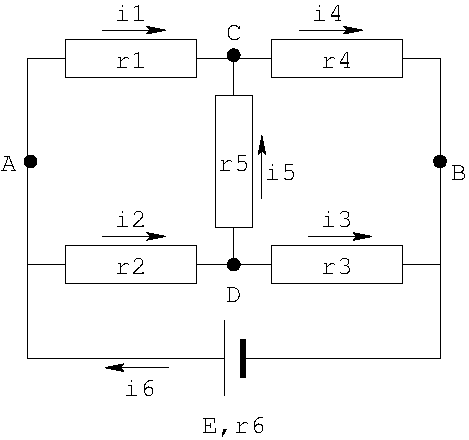
\includegraphics[width=6cm]{wheatstone.pdf}$$
$$
\begin{array}{lcr}
r_1 & = & 10 \Omega \\
r_2 & = & 10 \Omega \\
r_3 & = &  5 \Omega \\
r_4 & = & 20 \Omega \\
r_5 & = & 10 \Omega \\
r_6 & = & 10 \Omega \\
E   & = & 12 V 
\end{array}
\hspace*{5mm}
\left|\begin{array}{l}
i_4 = i_1 + i_5\\
i_6 = i_1 + i_2\\
i_2 = i_3 + i_5\\
10 i_1 = 10 i_2 + 10 i_5\\
10 i_5 = 5 i_3 - 20 i_4\\
12 - 10 i_6 = 10 i_2 + 5 i_3
\end{array}\right.
$$
\end{fig}

De nombreux exemples traités dans les enseignements scientifiques
conduisent à la nécessité de résoudre un système de $n$ équations linéaires
à $n$ inconnues, homogènes ou non homogènes, du type $A\cdot x = b$. 
La figure \ref{fig:wheatstone}
propose à titre d'exemple le cas du pont de Wheatstone en électricité.
Les ponts ont été utilisés pour la mesure des résistances, inductances et
capacités jusqu'à ce que les progrès en électronique les rendent obsolètes en
métrologie. Toutefois la structure en pont reste encore utilisée dans de 
nombreux montages.

La première méthode généralement utilisée pour trouver la solution 
d'un système d'équa\-tions linéaires tel que le système (\ref{eq1}) 
est celle qui consiste à éliminer les inconnues 
($x_i$) en combinant les équations.
Pour illustrer cette méthode, nous commencerons par étudier un exemple
simple pouvant s'effectuer {\em à la main}, 
puis nous passerons au cas général pour
présenter la méthode d'élimination de {\sc Gauss}.

%-------------------------------------------------------------------------
\subsection*{Etude d'un cas particulier}
\label{casparticulier}
%-------------------------------------------------------------------------
Considérons le système suivant :
$$\left\{
\begin{array}{rcrcrcr}
 x_0 & + &  x_1 & + &   x_2 & = &  1 \\
2x_0 & + & 4x_1 & + &  8x_2 & = & 10 \\
3x_0 & + & 9x_1 & + & 27x_2 & = & 33
\end{array}
\right.$$

Pour résoudre un tel système, l'idée de base est de triangulariser 
le système de telle manière qu'il soit possible de remonter les
solutions par substitutions successives.

La première étape consiste à éliminer le terme en $x_0$ des 
$2^{\grave eme}$ et $3^{\grave eme}$ équations.
Cherchons tout d'abord à éliminer le terme en $x_0$ de la $2^{\grave eme}$
équation. Pour cela nous multiplions la $1^{\grave ere}$ équation par le 
coefficient de $x_0$ de la $2^{\grave eme}$ équation ($a_{10} = 2$). 
On obtient le nouveau système :
$$\left\{
\begin{array}{rcrcrcr}
2x_0 & + & 2x_1 & + &  2x_2 & = &  2 \\
2x_0 & + & 4x_1 & + &  8x_2 & = & 10 \\
3x_0 & + & 9x_1 & + & 27x_2 & = & 33
\end{array}
\right.$$
On soustrait alors la première équation de la deuxième équation, 
ce qui conduit au système :
$$\left\{
\begin{array}{rcrcrcr}
2x_0 & + & 2x_1 & + &  2x_2 & = &  2 \\
     &   & 2x_1 & + &  6x_2 & = &  8 \\
3x_0 & + & 9x_1 & + & 27x_2 & = & 33
\end{array}
\right.$$
On recommence l'opération pour éliminer le terme en $x_0$ de la $3^{\grave eme}$
équation. Pour cela, on ramène à $1$ le coefficient de $x_0$ dans
la première équation en divisant cette équation par 2 ($a_{00} = 2$),
puis nous multiplions la $1^{\grave ere}$ équation par le 
coefficient de $x_0$ de la $3^{\grave eme}$ équation ($a_{20} = 3$). 
$$\left\{
\begin{array}{rcrcrcr}
3x_0 & + & 3x_1 & + &  3x_2 & = &  3 \\
     &   & 2x_1 & + &  6x_2 & = &  8 \\
3x_0 & + & 9x_1 & + & 27x_2 & = & 33
\end{array}
\right.$$
On soustrait ensuite la $1^{\grave ere}$ équation de la $3^{\grave eme}$ équation :
$$\left\{
\begin{array}{rcrcrcr}
3x_0 & + & 3x_1 & + &  3x_2 & = &  3 \\
     &   & 2x_1 & + &  6x_2 & = &  8 \\
     &   & 6x_1 & + & 24x_2 & = & 30
\end{array}
\right.$$
On obtient un nouveau système linéaire dans lequel seule la première équation contient
un terme en $x_0$.
L'équation utilisée (ici la $1^{\grave ere}$ équation) pour éliminer une inconnue 
dans les équations qui suivent (ici les $2^{\grave eme}$ et $3^{\grave eme}$ équations)
est appelée l'équation-pivot. Dans l'équation-pivot choisie, le coefficient de 
l'inconnue qui est éliminée dans les autres équations est appelé le pivot de
l'équation (ici $a_{00}$).

La deuxième étape consiste à éliminer le terme en $x_1$ de la troisième équation
en utilisant la deuxième équation comme équation-pivot. On ramène à $1$ le coefficient 
de $x_1$ dans la $2^{\grave eme}$ équation en divisant l'équation par 2 ($a_{11} = 2$),
puis on la multiplie par 6 ($a_{21} = 6$) pour que les $2^{\grave eme}$ et 
$3^{\grave eme}$ équations aient le même terme en $x_1$. Tout revient à
multiplier la $2^{\grave eme}$ équation par 3 ($a_{21}/a_{11} = 6/2 = 3$) :
$$\left\{
\begin{array}{rcrcrcr}
3x_0 & + & 3x_1 & + &  3x_2 & = &  3 \\
     &   & 6x_1 & + & 18x_2 & = & 24 \\
     &   & 6x_1 & + & 24x_2 & = & 30
\end{array}
\right.$$
Il reste à soustraire la $2^{\grave eme}$ équation de la $3^{\grave eme}$
pour éliminer le terme en $x_1$ de la $3^{\grave eme}$ équation :
$$\left\{
\begin{array}{rcrcrcr}
3x_0 & + & 3x_1 & + &  3x_2 & = &  3 \\
     &   & 6x_1 & + & 18x_2 & = & 24 \\
     &   &      &   &  6x_2 & = &  6
\end{array}
\right.$$
On obtient ainsi un système triangulaire d'équations linéaires 
dont on peut calculer
directement la valeur de $x_2$ par la $3^{\grave eme}$ équation : $6x_2 =  6 \Rightarrow
x_2 = 1$. On porte cette valeur de $x_2$ dans la deuxième équation, ce qui nous permet de
calculer $x_1$ : $6x_1 + 18\cdot 1 = 24 \Rightarrow x_1 = 1$. En reportant les valeurs de
$x_2$ et $x_1$ dans la première équation, on en déduit la valeur de $x_0$ :
$3x_0 + 3\cdot 1 +  3\cdot 1 =  3 \Rightarrow x_0 = -1$. 
On vérifie simplement que
les valeurs obtenues sont solutions du système initial :
$$\left\{
\begin{array}{rcrcrcr}
 x_0 & + &  x_1 & + &   x_2 & = &  1 \\
2x_0 & + & 4x_1 & + &  8x_2 & = & 10 \\
3x_0 & + & 9x_1 & + & 27x_2 & = & 33
\end{array}
\right.
\hspace*{2cm}
\left(
\begin{array}{rrr}
1 & 1 &  1 \\
2 & 4 &  8 \\
3 & 9 & 27 
\end{array}
\right)
\cdot
\left(
\begin{array}{r}
-1 \\ 1 \\ 1
\end{array}
\right)
=
\left(
\begin{array}{r}
1 \\ 10 \\ 33
\end{array}
\right)$$

%-------------------------------------------------------------------------
\subsection*{Etude du cas général}
\label{casgeneral}
%-------------------------------------------------------------------------
De manière générale, la méthode précédente consiste à réduire le système de $n$ 
équations à $n$ inconnues à un système triangulaire équivalent qui peut 
être ensuite résolu facilement par substitutions. En quelque sorte le système 
(\ref{eq1}) doit être transformé en un système équivalent du type :
\begin{equation}\label{eq2}
\left\{
\begin{array}{rcrcrcrcr@{\ =\ }r}
a_{00}x_0 &+& a_{01}x_1       &+& a_{02}x_2       &+& \cdots &+& a_{0(n-1)}x_{(n-1)}       & b_0\\
          & & a^{(1)}_{11}x_1 &+& a^{(1)}_{12}x_2 &+& \cdots &+& a^{(1)}_{1(n-1)}x_{(n-1)} & b^{(1)}_1\\
          & &                 &+& a^{(2)}_{22}x_2 &+& \cdots &+& a^{(2)}_{2(n-1)}x_{(n-1)} & b^{(2)}_2\\
          & &                 & &                 & & \cdots &+& \cdots           & \cdots\\
          & &                 & &                 & &        & & a^{(n-2)}_{(n-1)(n-1)}x_{(n-1)}   & b^{(n-2)}_{(n-1)}
\end{array}
\right.
\end{equation}
où l'indice supérieur désigne le nombre d'étapes à la suite desquelles est obtenu le 
coefficient considéré.

L'équation de rang 0 du système (\ref{eq1}) est d'abord divisée par le coefficient 
$a_{00}$ de $x_0$ (supposé non nul). On obtient :
\begin{equation}\label{eq3}
x_0 + \frac{a_{01}}{a_{00}}x_1 + \frac{a_{02}}{a_{00}}x_2 + \cdots + \frac{a_{0(n-1)}}{a_{00}}x_{(n-1)} = \frac{b_0}{a_{00}}
\end{equation}
Cette équation (\ref{eq3}) est alors multiplié par $a_{10}$, coefficient de $x_0$ dans 
la deuxième équation du système (\ref{eq1}). Le résultat est ensuite soustrait de la 
deuxième équation du système (\ref{eq1}), ce qui élimine $x_0$ dans la deuxième équation.
D'une manière générale on multiplie la relation (\ref{eq3}) par $a_{i0}$, coefficient
de $x_0$ dans l'équation de rang $i$ du système (\ref{eq1}) et on retranche le résultat
obtenu de cette même $i^{\grave eme}$ équation. A la fin $x_0$ est éliminé de toutes les équations, excepté de la première, et on obtient le système ainsi transformé :
\begin{equation}\label{eq4}
\left\{
\begin{array}{rcrcrcrcr@{\ =\ }r}
a_{00}x_0 &+& a_{01}x_1       &+& a_{02}x_2       &+& \cdots &+& a_{0(n-1)}x_{(n-1)}       & b_0\\
          & & a^{(1)}_{11}x_1 &+& a^{(1)}_{12}x_2 &+& \cdots &+& a^{(1)}_{1(n-1)}x_{(n-1)} & b^{(1)}_1\\
          & & a^{(1)}_{21}x_1 &+& a^{(1)}_{22}x_2 &+& \cdots &+& a^{(1)}_{2(n-1)}x_{(n-1)} & b^{(1)}_2\\
          & & a^{(1)}_{31}x_1 &+& a^{(1)}_{32}x_2 &+& \cdots &+& a^{(1)}_{3(n-1)}x_{(n-1)} & b^{(1)}_3\\
          & & \cdots          &+& \cdots          &+& \cdots &+& \cdots                    & \cdots\\
          & & a^{(1)}_{(n-1)1}x_1 &+& a^{(1)}_{(n-1)2}x_2 &+& \cdots &+& a^{(1)}_{(n-1)(n-1)}x_{(n-1)}   & b^{(1)}_{(n-1)}
\end{array}
\right.
\end{equation}
L'équation de rang 1 dans le nouveau système (\ref{eq4}) devient alors l'équation-pivot
et $a^{(1)}_{11}$ le pivot de l'équation. De la même façon on élimine $x_1$ des
équations du rang $2$ au rang $n-1$ dans le système (\ref{eq4}), et on obtient :
\begin{equation}\label{eq5}
\left\{
\begin{array}{rcrcrcrcr@{\ =\ }r}
a_{00}x_0 &+& a_{01}x_1       &+& a_{02}x_2       &+& \cdots &+& a_{0(n-1)}x_{(n-1)}       & b_0\\
          & & a^{(1)}_{11}x_1 &+& a^{(1)}_{12}x_2 &+& \cdots &+& a^{(1)}_{1(n-1)}x_{(n-1)} & b^{(1)}_1\\
          & &                 & & a^{(2)}_{22}x_2 &+& \cdots &+& a^{(2)}_{2(n-1)}x_{(n-1)} & b^{(2)}_2\\
          & &                 & & a^{(2)}_{32}x_2 &+& \cdots &+& a^{(2)}_{3(n-1)}x_{(n-1)} & b^{(2)}_3\\
          & &                 & & \cdots          &+& \cdots &+& \cdots                    & \cdots\\
          & &                 & & a^{(2)}_{(n-1)2}x_2 &+& \cdots &+& a^{(2)}_{(n-1)(n-1)}x_{(n-1)}   & b^{(2)}_{(n-1)}
\end{array}
\right.
\end{equation}
L'équation de rang 2 dans le nouveau système (\ref{eq5}) fait office à son tour d'équation
pivot, et ainsi de suite jusqu'à obtenir le système triangulaire (\ref{eq2}).
Une fois obtenu ce système triangulaire, on calcule directement
la valeur de $x_{(n-1)}$ par la dernière relation du système triangulaire. 
En portant cette valeur dans la relation précédente, on calculera
$x_{(n-2)}$, et ainsi de suite en remontant le système triangulaire (\ref{eq2}).
A chaque étape $k$, on a donc les relations suivantes :
\begin{enumerate}
\item {Triangularisation}
	$$\left\{
	\begin{array}{lcl}
	a_{ij}^{(k)} & = & \displaystyle a_{ij}^{(k-1)} - \frac{a_{ip}^{(k-1)}}{a_{pp}^{(k-1)}}\cdot
	a_{pj}^{(k-1)} \\[5mm]
	b_i^{(k)}    & = & \displaystyle b_i^{(k-1)} - \frac{a_{ip}^{(k-1)}}{a_{pp}^{(k-1)}}\cdot
	b_p^{(k-1)}
	\end{array}
	\right.\mbox{\footnotesize\ avec\ }
	\left\{
	\begin{array}{l}
	k\ :\ \mbox{\footnotesize étape}\\
	p\ : \ \mbox{\footnotesize rang du pivot}\\[5mm]
	p < i \leq (n-1) \\[2mm]
	p \leq j \leq (n-1)
	\end{array}
	\right.$$
\item {Remontée par substitutions} 
	$$\left\{
	\begin{array}{lcl}
	x_{(n-1)} & = & \displaystyle\frac{b_{(n-1)}}{a_{(n-1)(n-1)}}\\[5mm]
	x_i       & = & \displaystyle\frac{\displaystyle b_{i} - 
	\sum_{j=i+1}^{n-1} a_{ij}x_j}{a_{ii}} 
	\end{array}
	\right.
	\mbox{\ avec\ } 0 \leq i < (n-1)$$
\end{enumerate}

Jusqu'à présent, on a admis que le pivot au cours du processus de triangularisation 
était non nul ($a_{pp} \neq 0$). Si ce n'est pas le cas, on doit permuter 
l'équation-pivot avec une autre ligne dans laquelle le pivot est différent de 0.
Il se peut également que le pivot, sans être nul, soit très petit et l'on a 
intérêt là-aussi à interchanger les lignes comme pour le cas d'un pivot nul.
En fait, pour augmenter la précision de la solution obtenue, on a toujours 
intérêt à utiliser la ligne qui a le plus grand pivot.

Cette méthode est connue sous le nom de méthode d'élimination 
de {\sc Gauss} (également connue sous
le nom de méthode de triangularisation de {\sc Gauss} ou méthode du pivot 
de {\sc Gauss}). Elle fut nommée ainsi en l'honneur du mathématicien allemand 
{\sc Johann Carl Friedrich Gauss} (1777--1855), mais elle est connue des Chinois 
depuis au moins le $1^{er}$ siècle de notre ère. Elle est référencée dans le livre 
chinois « Jiuzhang suanshu~» où elle est attribuée à {\sc Chang Ts'ang} chancelier de 
l'empereur de Chine au $2^{\grave eme}$ siècle avant notre ère. 


%-------------------------------------------------------------------------
\subsection*{Jeu de tests}
%-------------------------------------------------------------------------
L'algorithme de résolution de tels systèmes linéaires pourra être testé
à l'aide des systèmes suivants :
$$\begin{array}{|l|c|c|c|}
\hline
\mbox{\bf Test} & \multicolumn{2}{|c|}{\mbox{{\bf Système} $A\cdot x = b$}} & \bf Solution\\
\cline{2-3}
                & A & b & \bf exacte \\
\hline
\hline
1 
& 
\left(\begin{array}{r}
4
\end{array}\right) 
&
\left(\begin{array}{r}
1
\end{array}\right) 
&
\displaystyle
\left(\begin{array}{r}
1/4
\end{array}\right)\\
\hline
2 
& 
\left(\begin{array}{rr}
1 & 1 \\
1 & -1
\end{array}\right) 
&
\left(\begin{array}{r}
1 \\ 0
\end{array}\right)
&
\displaystyle
\left(\begin{array}{r}
1/2 \\ 1/2
\end{array}\right)
\\
\hline
3 
& 
\left(\begin{array}{rrr}
2 & -1 & 2 \\
1 & 10 & -3 \\
-1 & 2 & 1
\end{array}\right) 
&
\left(\begin{array}{r}
2 \\ 5 \\ -3
\end{array}\right)
&
\left(\begin{array}{r}
2 \\ 0 \\ -1
\end{array}\right)
\\
\hline
\end{array}$$


$$\begin{array}{|l|c|c|c|}
\hline
\mbox{\bf Test} & \multicolumn{2}{|c|}{\mbox{{\bf Système} $A\cdot x = b$}} & \bf Solution\\
\cline{2-3}
                & A & b & \bf exacte \\
\hline
4 &
\left(\begin{array}{rrrr}
10 & 7 & 8 & 7 \\
7 & 5 & 6 & 5 \\
8 & 6 & 10 & 9 \\
7 & 5 & 9 & 10
\end{array}\right) 
&
\left(\begin{array}{r}
32 \\ 23 \\ 33 \\ 31
\end{array}\right) 
&
\left(\begin{array}{r}
1 \\ 1 \\ 1 \\ 1
\end{array}\right) 
\\
\hline
5 & 
\left(\begin{array}{rrrr}
10 & 7 & 8.1 & 7.2 \\
7.08 & 5.04 & 6 & 5 \\
8 & 5.98 & 9.89 & 9 \\
6.99 & 4.99 & 9 & 9.98
\end{array}\right) 
&
\left(\begin{array}{r}
32 \\ 23 \\ 33 \\ 31
\end{array}\right) 
&
\mbox{---} \\
\hline
6 &
\left(\begin{array}{rrrr}
10 & 7 & 8 & 7 \\
7 & 5 & 6 & 5 \\
8 & 6 & 10 & 9 \\
7 & 5 & 9 & 10
\end{array}\right) 
&
\left(\begin{array}{r}
32.01 \\ 22.99 \\ 33.01 \\ 30.99
\end{array}\right) 
&
\mbox{---} \\
\hline
\end{array}$$

Les tests 5 et 6 sont des variations du test 4 : $A_5 = A_4 + \Delta A$
et $b_6 = b_4 + \Delta b$. Ces 2 tests sont effectués pour évaluer 
les conséquences sur la solution $x$ d'une perturbation $\Delta A$ de $A_4$
et d'une perturbation $\Delta b$ de $b_4$.
$$\Delta A = \left(\begin{array}{rrrr}
0 & 0 & 0.1 & 0.2\\
0.08 & 0.04 & 0 & 0\\
0 & -0.02 & -0.11 & 0\\
-0.01 & -0.01 & 0 & -0.02
\end{array}
\right)$$
$$\Delta b = \left(\begin{array}{r}
0.01 \\ - 0.01 \\ 0.01 \\ -0.01
\end{array}\right)$$
$$\begin{array}{|l|c|c|}
\hline
\mbox{\bf Test} & \multicolumn{2}{|c|}{\mbox{{\bf Système} $A\cdot x = b$}}\\
\cline{2-3}
                & A & b  \\
\hline
\hline
7 &
\left(\begin{array}{rrrrrr}
1 & 0 & 0 & - & 1 & 0\\
1 & 1 & 0 & 0 & 0 & -1\\
0 & 1 & -1 & 0 & -1 & 0\\
10 & -10 & 0 & 0 & -10 & 0\\
0 & 0 & 5 & -20 & -10 & 0\\
0 & 10 & 5 & 0 & 0 & 10
\end{array}\right) 
&
\left(\begin{array}{r}
0 \\ 0 \\ 0 \\ 0 \\ 0 \\ 12
\end{array}\right)\\
\hline
8 &
\left(\begin{array}{rrrrrrrr}
1 & 0 & 0 & 0 & 0 & 0 & 0 & 0\\
1 & 2\pi & 4\pi^2 & 8\pi^3 & 16\pi^4 & 32\pi^5 & 64\pi^6 & 128\pi^7\\
0 & 1 & 0 & 0 & 0 & 0 & 0 & 0\\
0 & 1 & 4\pi & 12\pi^2 & 32\pi^3 & 80\pi^4 & 192\pi^5 & 448\pi^6\\
1 & \pi/2 & \pi^2/4 & \pi^3/8 & \pi^4/16 & \pi^5/32 & \pi^6/64 & \pi^7/128\\
0 & \pi/2 & \pi & 3\pi^2/4 & \pi^3/2 & 5\pi^4/16 & 3\pi^5/16 & 7\pi^6/64\\
1 & \pi & \pi^2 & \pi^3 & \pi^4 & \pi^5 & \pi^6 & \pi^7\\
0 & \pi & 2\pi & 3\pi^2 & 4\pi^3 & 5\pi^4 & 6\pi^5 & 7\pi^6
\end{array}\right) 
&
\left(\begin{array}{r}
4 \\ 4 \\ 0 \\ 0 \\ 2 \\ -2 \\ 1 \\ 0
\end{array}\right)\\
\hline
\end{array}$$


Le test 7 correspond à l'exemple du pont de Wheatstone 
(figure \ref{fig:wheatstone}). Le test 8 correspond
à la détermination de la forme d'une came rotative qui doit
mettre en mouvement un axe suivant une loi horaire donnée.

%-------------------------------------------------------------------------

%-------------------------------------------------------------------------
\chapter*{Liste des exercices}
\addcontentsline{toc}{chapter}{Liste des exercices}
	\listtheorems{td}
%-------------------------------------------------------------------------


\label{fin}
%-------------------------------------------------------------------------
\end{document}
%-------------------------------------------------------------------------
